\documentclass[12pt,letterpaper]{article}
\usepackage[utf8]{inputenc}
\usepackage[spanish]{babel}
\usepackage[margin=2.5cm]{geometry}
\usepackage{graphicx}
\usepackage{listings}
\usepackage{xcolor}
\usepackage{hyperref}
\usepackage{float}
\usepackage{amsmath}

\definecolor{codegreen}{rgb}{0,0.6,0}
\definecolor{codegray}{rgb}{0.5,0.5,0.5}
\definecolor{codepurple}{rgb}{0.58,0,0.82}
\definecolor{backcolour}{rgb}{0.96,0.96,0.94}

\lstdefinestyle{mystyle}{
    backgroundcolor=\color{backcolour},   
    commentstyle=\color{codegreen},
    keywordstyle=\color{magenta},
    numberstyle=\tiny\color{codegray},
    stringstyle=\color{codepurple},
    basicstyle=\ttfamily\scriptsize,
    breakatwhitespace=false,         
    breaklines=true,                 
    captionpos=b,                    
    keepspaces=true,                 
    numbers=left,                    
    numbersep=5pt,                  
    showspaces=false,                
    showstringspaces=false,
    showtabs=false,                  
    tabsize=2
}

\lstset{style=mystyle}

\hypersetup{
    colorlinks=true,
    linkcolor=blue,
    filecolor=magenta,      
    urlcolor=blue,
    citecolor=blue
}

\begin{document}

% --- Portada / Encabezado ---
\begin{center}
    
\includegraphics[width=0.25\textwidth]{figuras/logo_unal.png} \\[0.4cm]
    {\Large \textbf{UNIVERSIDAD NACIONAL DE COLOMBIA}} \\[0.3cm]
    {\large \textbf{FACULTAD DE MINAS -- SEDE MEDELLÍN}} \\[0.2cm]
    {\large \textbf{PROGRAMACIÓN ORIENTADA A OBJETOS -- SEMESTRE 2026-2S}} \\[0.5cm]
    {\Large \textbf{ACTIVIDAD 4: EXCEPCIONES Y ENTRADA/SALIDA CON INTERFAZ GRÁFICA}} \\[0.8cm]
    
    \textbf{Docente:} \\
    Walter Hugo Arboleda Mazo \\[0.5cm]

    \textbf{Estudiante:} \\
    Yuliana Stefania Guzmán Montoya -- C.C. 1.001.765.162 \\[0.8cm]

    Medellín, Colombia \\
    Noviembre de 2026
\end{center}

\vspace{0.8cm}
\hrule
\vspace{0.8cm}

% ==============================================================================
% EJERCICIO 1
% ==============================================================================
\section{Ejercicio Página 400 (Ejercicio 6.4: Excepciones)}

\noindent\textbf{Enlace a GitHub:} \\
\url{https://github.com/yguzmanm-sys/POO-2026-2S/blob/main/Actividad4/Ejercicio6_4.py}

\subsection{Descripción del Problema}
El ejercicio 6.4 del texto guía aborda el funcionamiento de las estructuras de control de excepciones basadas en los bloques \texttt{try}, \texttt{catch} (denominado \texttt{except} en Python) y \texttt{finally}. El objetivo es estudiar la separación entre el flujo normal de ejecución y el tratamiento de condiciones anómalas (como la división por cero con \texttt{ZeroDivisionError} o el acceso a métodos de referencias nulas con \texttt{AttributeError}), garantizando que el bloque \texttt{finally} se ejecute de manera incondicional. Para esta actividad se diseñó una solución con interfaz gráfica interactiva que permite ingresar operandos, simular los errores descritos en el libro y registrar la traza de ejecución paso a paso.

\subsection{Código Fuente}

\begin{lstlisting}[language=Python, caption=Implementación del Ejercicio 6.4 en Python, label=lst:ej64]
import tkinter as tk
from tkinter import ttk, messagebox, scrolledtext

class OperacionesExcepciones:
    def __init__(self):
        self.registro = []

    def log(self, mensaje: str):
        self.registro.append(mensaje)

    def ejecutar_division(self, num_str: str, den_str: str) -> tuple[float | None, list[str]]:
        self.registro = []
        resultado = None
        self.log("Ingresando al bloque try de division.")
        try:
            num = float(num_str)
            den = float(den_str)
            resultado = num / den
            self.log(f"Division exitosa: {num} / {den} = {resultado}")
        except ZeroDivisionError as e:
            self.log("Excepcion capturada: ZeroDivisionError (Division por cero).")
            raise ZeroDivisionError("No es posible dividir por cero.") from e
        except ValueError as e:
            self.log("Excepcion capturada: ValueError (Los valores deben ser numericos).")
            raise ValueError("Ingrese valores numericos validos.") from e
        finally:
            self.log("Ingresando al bloque finally de division (se ejecuta siempre).")
        return resultado, self.registro

    def ejecutar_objeto_nulo(self) -> list[str]:
        self.registro = []
        self.log("Ingresando al bloque try de acceso a objeto.")
        try:
            objeto = None
            self.log("Intentando llamar metodo sobre objeto None.")
            objeto.metodo_inexistente()
        except AttributeError as e:
            self.log("Excepcion capturada: AttributeError (Objeto nulo no tiene atributos).")
            raise AttributeError("Intento de acceso a miembro de un objeto None.") from e
        except Exception as e:
            self.log("Excepcion capturada: Exception general.")
            raise Exception("Ocurrio una excepcion general.") from e
        finally:
            self.log("Ingresando al bloque finally de objeto (se ejecuta siempre).")
        return self.registro


class VentanaExcepciones(tk.Tk):
    def __init__(self):
        super().__init__()
        self.title("Ejercicio 6.4 - Manejo de Excepciones")
        self.geometry("520x540")
        self.resizable(False, False)
        self.operaciones = OperacionesExcepciones()
        self._construir_ui()

    def _construir_ui(self):
        marco_principal = ttk.Frame(self, padding="15")
        marco_principal.pack(fill=tk.BOTH, expand=True)

        lbl_titulo = ttk.Label(marco_principal, text="Demostracion de Bloques Try - Catch - Finally", font=("Segoe UI", 13, "bold"))
        lbl_titulo.pack(pady=(0, 15))

        marco_campos = ttk.LabelFrame(marco_principal, text="Division Aritmetica", padding="10")
        marco_campos.pack(fill=tk.X, pady=5)

        ttk.Label(marco_campos, text="Numerador:").grid(row=0, column=0, sticky=tk.W, pady=3)
        self.txt_numerador = ttk.Entry(marco_campos, width=15)
        self.txt_numerador.grid(row=0, column=1, sticky=tk.W, padx=5, pady=3)
        self.txt_numerador.insert(0, "10000")

        ttk.Label(marco_campos, text="Denominador:").grid(row=1, column=0, sticky=tk.W, pady=3)
        self.txt_denominador = ttk.Entry(marco_campos, width=15)
        self.txt_denominador.grid(row=1, column=1, sticky=tk.W, padx=5, pady=3)
        self.txt_denominador.insert(0, "0")

        marco_botones = ttk.Frame(marco_principal)
        marco_botones.pack(fill=tk.X, pady=10)

        btn_dividir = ttk.Button(marco_botones, text="Ejecutar Division", command=self._accion_dividir)
        btn_dividir.pack(side=tk.LEFT, padx=3)

        btn_nulo = ttk.Button(marco_botones, text="Probar Objeto Nulo", command=self._accion_objeto_nulo)
        btn_nulo.pack(side=tk.LEFT, padx=3)

        btn_limpiar = ttk.Button(marco_botones, text="Limpiar Consola", command=self._accion_limpiar)
        btn_limpiar.pack(side=tk.LEFT, padx=3)

        ttk.Label(marco_principal, text="Traza de Ejecucion (Consola):", font=("Segoe UI", 10, "bold")).pack(anchor=tk.W, pady=(5, 2))
        self.txt_consola = scrolledtext.ScrolledText(marco_principal, width=58, height=14, font=("Consolas", 9))
        self.txt_consola.pack(fill=tk.BOTH, expand=True)

    def _imprimir_consola(self, lineas: list[str], es_error: bool = False, msg_error: str = ""):
        for linea in lineas:
            self.txt_consola.insert(tk.END, f"> {linea}\n")
        if es_error:
            self.txt_consola.insert(tk.END, f"[ERROR GESTIONADO]: {msg_error}\n")
        self.txt_consola.insert(tk.END, "-" * 55 + "\n")
        self.txt_consola.see(tk.END)

    def _accion_dividir(self):
        num = self.txt_numerador.get().strip()
        den = self.txt_denominador.get().strip()
        try:
            _, reg = self.operaciones.ejecutar_division(num, den)
            self._imprimir_consola(reg)
        except (ZeroDivisionError, ValueError) as err:
            self._imprimir_consola(self.operaciones.registro, es_error=True, msg_error=str(err))
            messagebox.showerror("Error de Ejecucion", str(err))

    def _accion_objeto_nulo(self):
        try:
            reg = self.operaciones.ejecutar_objeto_nulo()
            self._imprimir_consola(reg)
        except (AttributeError, Exception) as err:
            self._imprimir_consola(self.operaciones.registro, es_error=True, msg_error=str(err))
            messagebox.showwarning("Excepcion de Objeto", str(err))

    def _accion_limpiar(self):
        self.txt_consola.delete("1.0", tk.END)


if __name__ == "__main__":
    app = VentanaExcepciones()
    app.mainloop()
\end{lstlisting}

\subsection{Interfaz de usuario}
La figura \ref{fig:ui_64} muestra la interfaz gráfica de usuario desarrollada. Esta contiene controles para ingresar el numerador y denominador de la división, botones para disparar tanto la división como la prueba de acceso a objeto nulo, y un área de consola interna que despliega en tiempo real la secuencia exacta de mensajes producidos por los bloques \texttt{try}, \texttt{catch} y \texttt{finally}.

\begin{figure}[H]
    \centering
    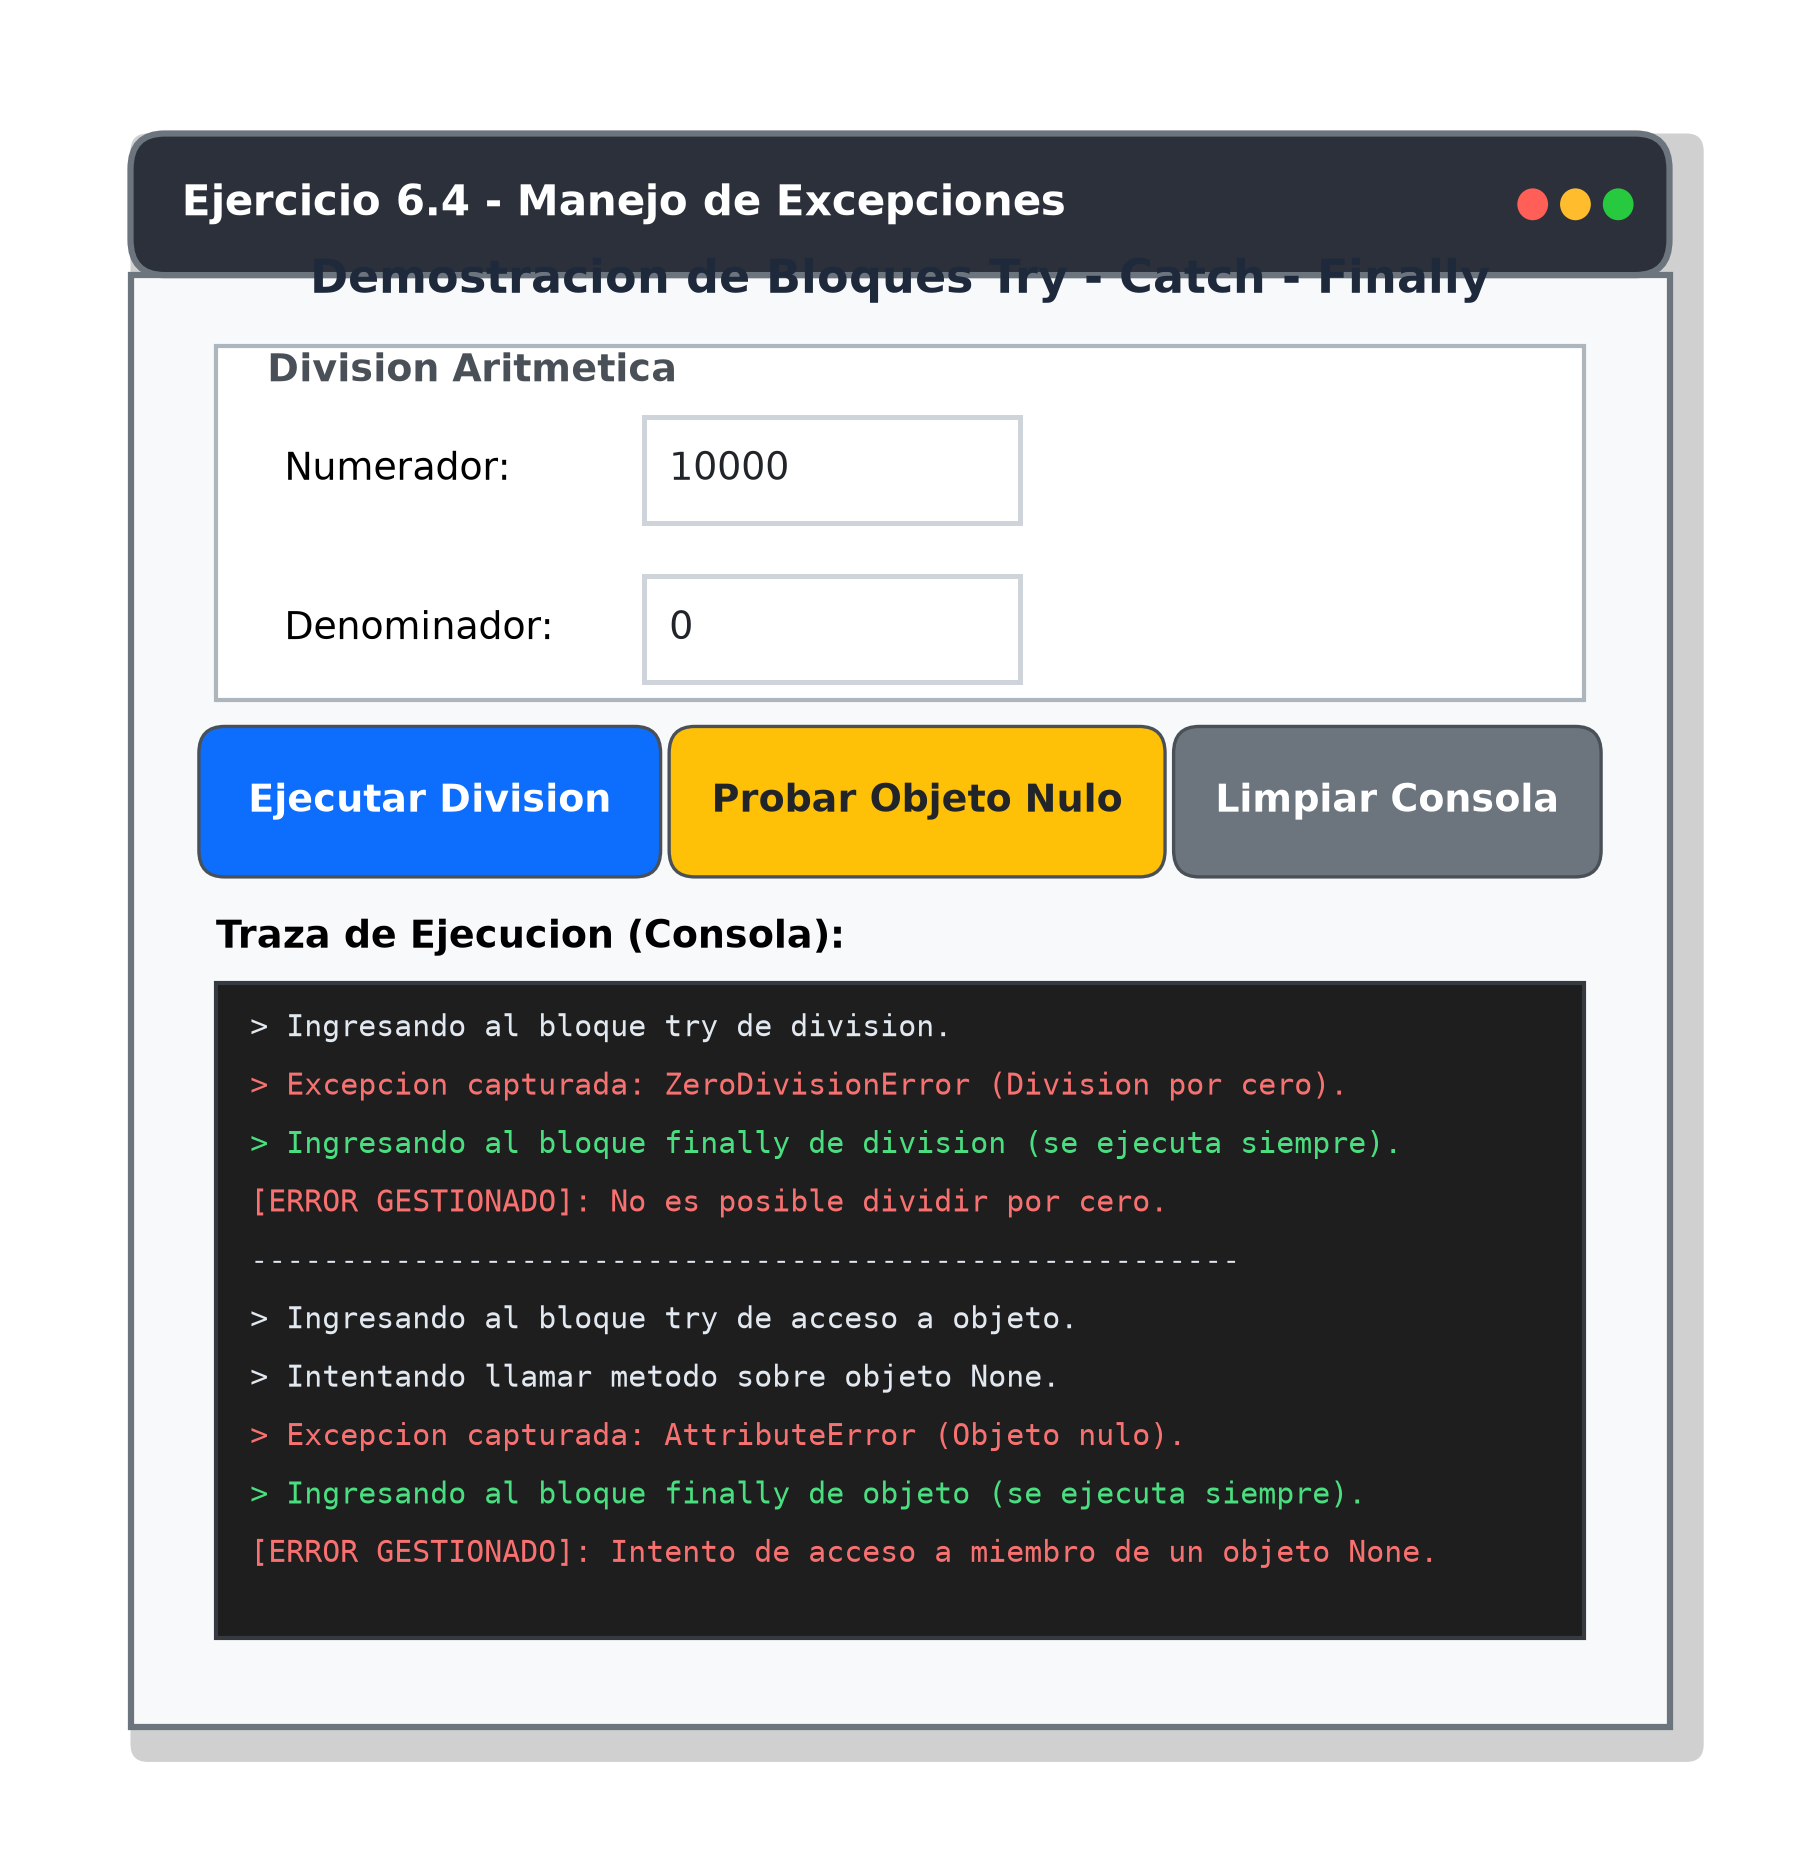
\includegraphics[width=0.55\textwidth]{figuras/ui_ejercicio6_4.png}
    \caption{Interfaz de usuario para el ejercicio 6.4 (Página 400).}
    \label{fig:ui_64}
\end{figure}

\subsection{Diagramas UML}

\subsubsection{Diagrama de clases}
El diagrama de clases de la figura \ref{fig:clases_64} modela la arquitectura orientada a objetos de la solución. La clase \texttt{OperacionesExcepciones} encapsula la lógica de cálculo y la traza de eventos de cada bloque de control. La clase \texttt{VentanaExcepciones} gestiona la interfaz gráfica y se comunica con la lógica mediante una relación de asociación y uso.

\begin{figure}[H]
    \centering
    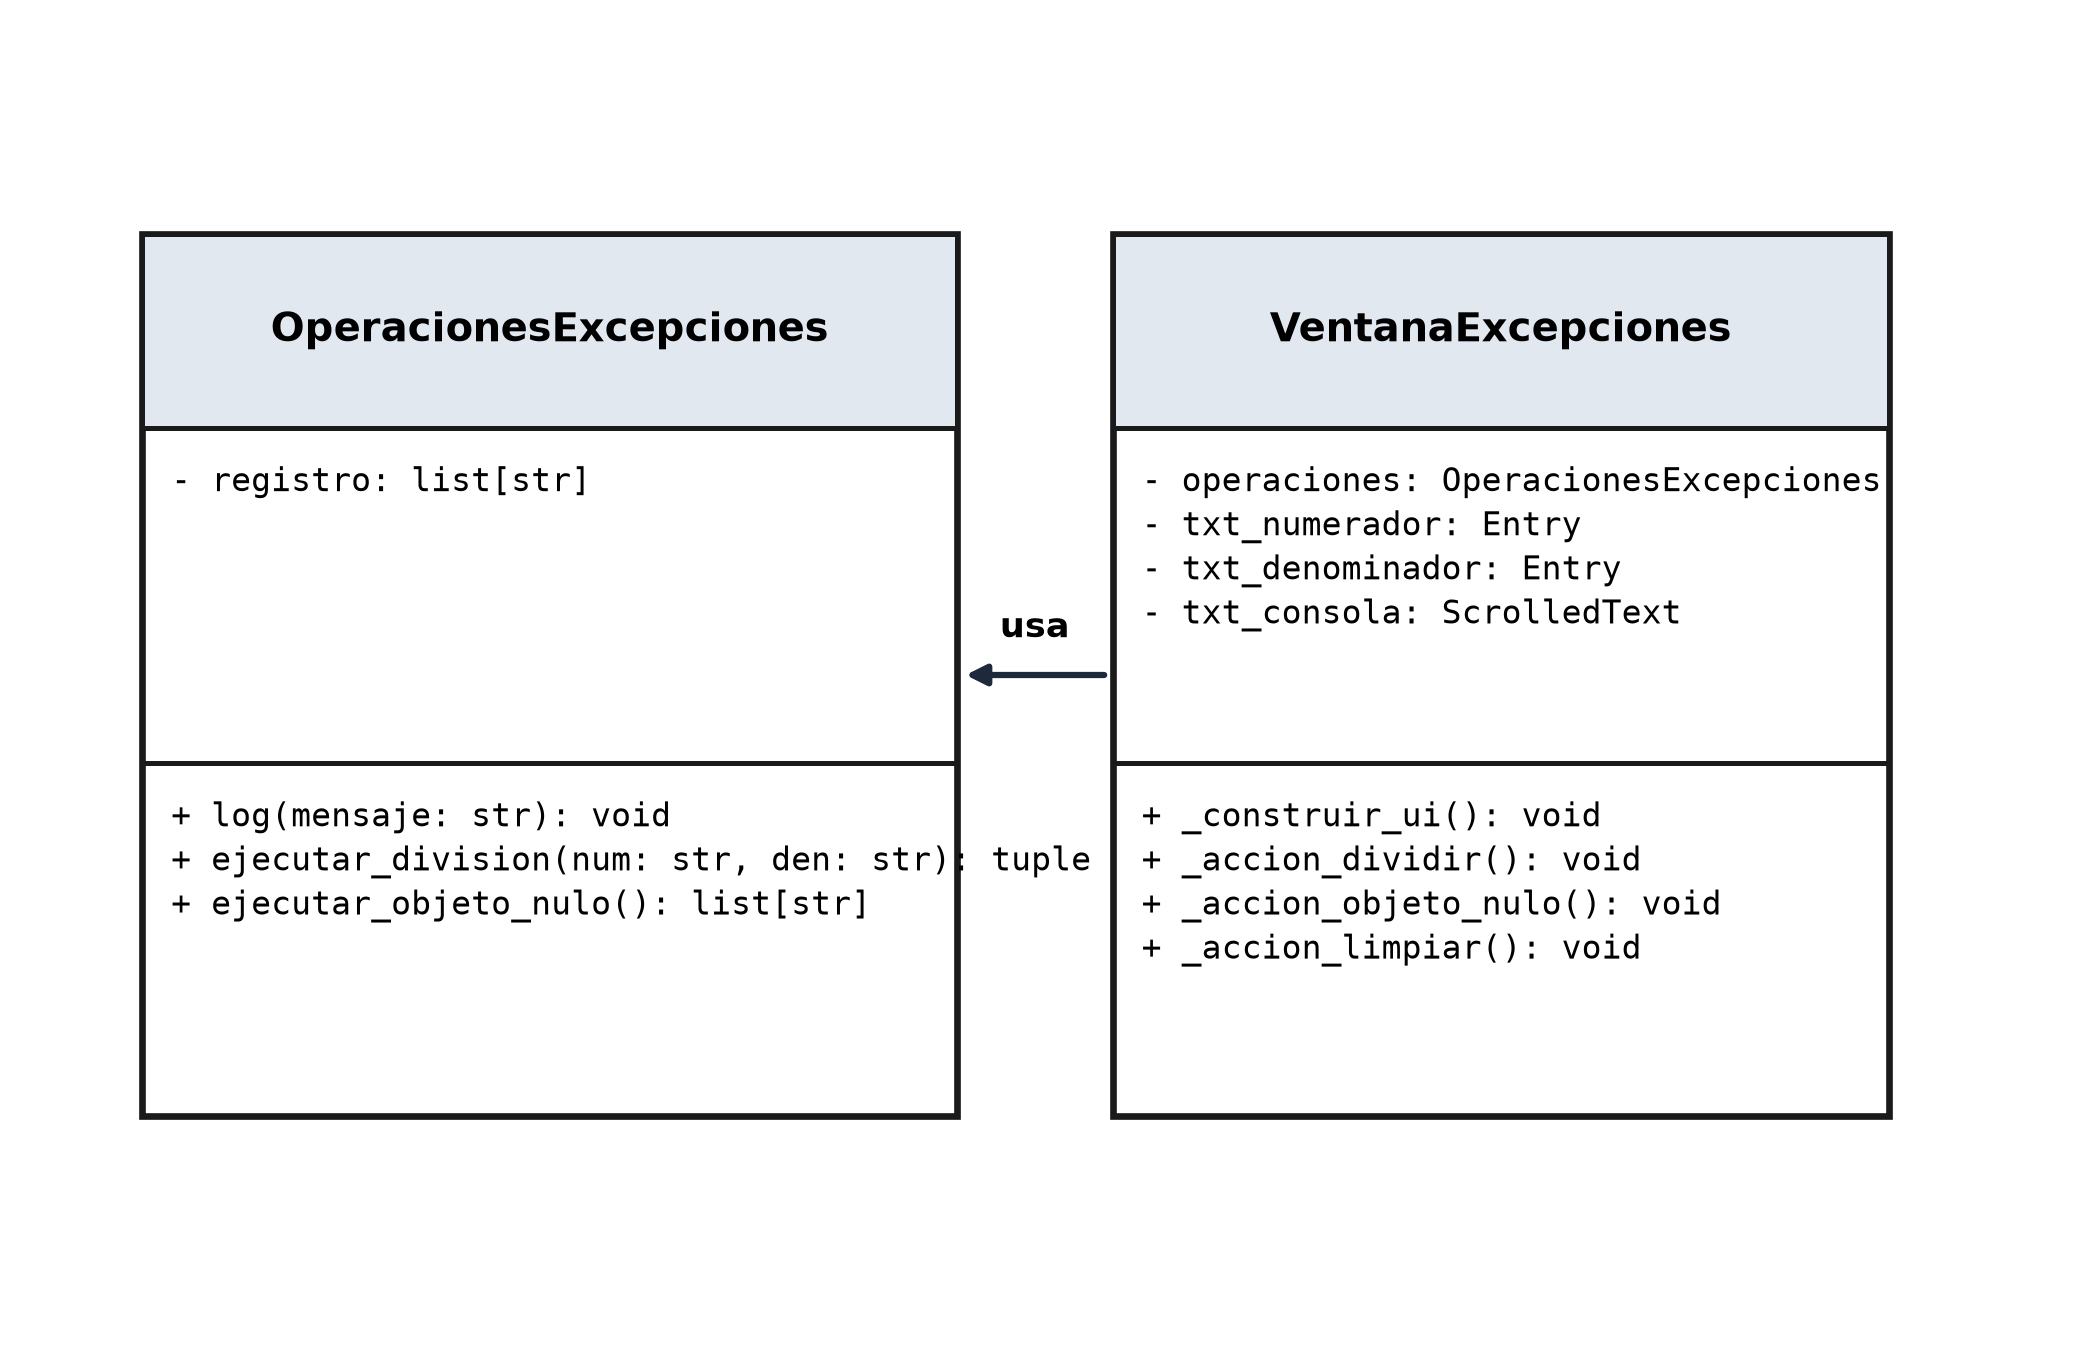
\includegraphics[width=0.78\textwidth]{figuras/clases_ejercicio6_4.png}
    \caption{Diagrama de clases para el ejercicio 6.4.}
    \label{fig:clases_64}
\end{figure}

\subsubsection{Casos de uso}
La figura \ref{fig:casos_64} expone las principales interacciones del usuario con la aplicación.

\begin{figure}[H]
    \centering
    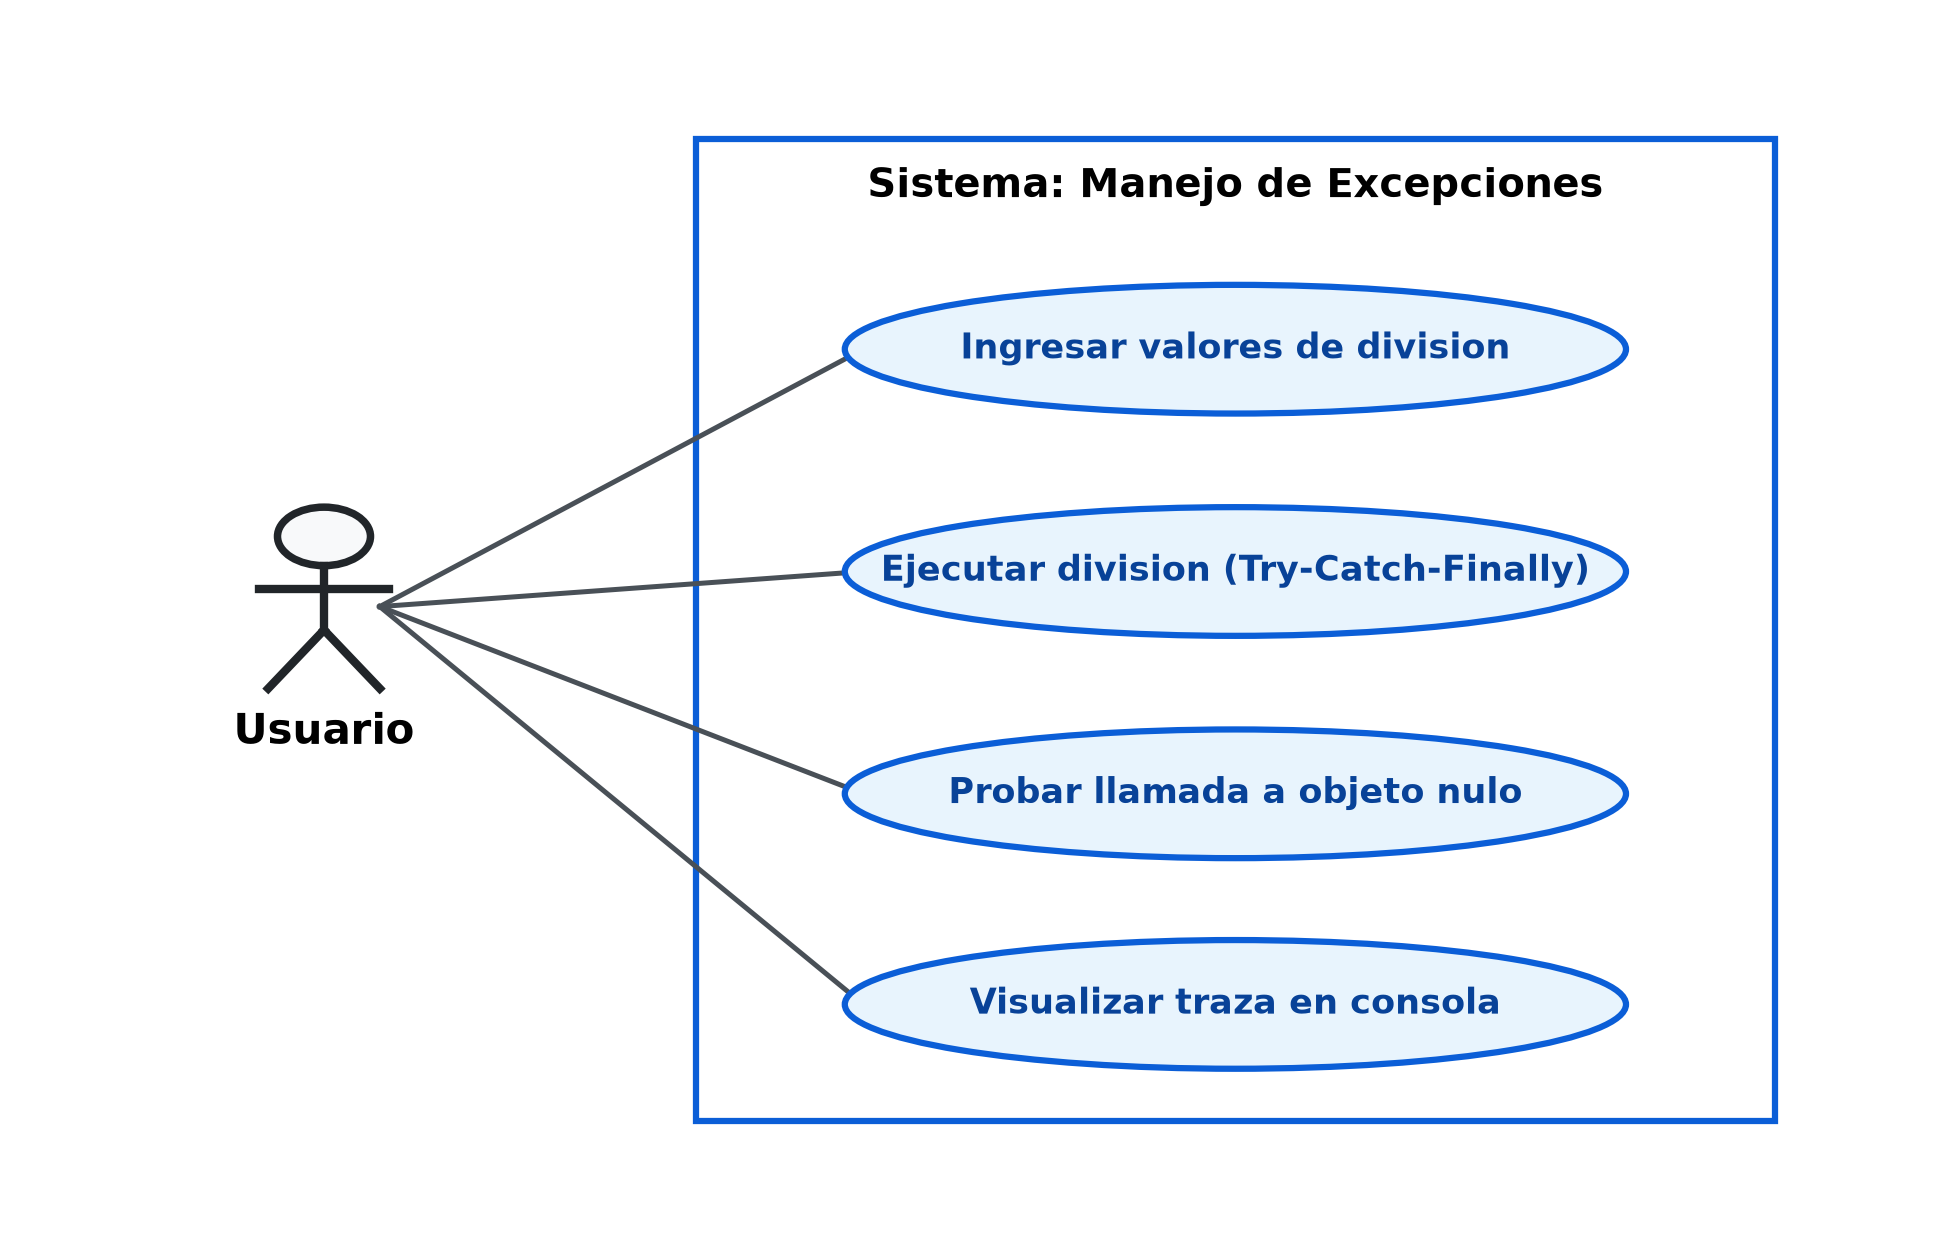
\includegraphics[width=0.75\textwidth]{figuras/casos_ejercicio6_4.png}
    \caption{Diagrama de casos de uso para el ejercicio 6.4.}
    \label{fig:casos_64}
\end{figure}

\begin{itemize}
    \item \textbf{Ingresar valores de división:} el usuario suministra el numerador y el denominador a través de las cajas de texto.
    \item \textbf{Ejecutar división (Try-Catch-Finally):} desencadena el procesamiento matemático, interceptando la división por cero si el denominador es nulo.
    \item \textbf{Probar llamada a objeto nulo:} evalúa la captura de excepciones generadas al acceder a miembros inexistentes de una referencia \texttt{None}.
    \item \textbf{Visualizar traza en consola:} permite verificar visualmente el orden incondicional de los bloques \texttt{finally}.
\end{itemize}

\clearpage

% ==============================================================================
% EJERCICIO 2
% ==============================================================================
\section{Ejercicio Página 406 (Ejercicio 6.5: Lanzamiento de excepciones)}

\noindent\textbf{Enlace a GitHub:} \\
\url{https://github.com/yguzmanm-sys/POO-2026-2S/blob/main/Actividad4/Ejercicio6_5.py}

\subsection{Descripción del Problema}
El ejercicio 6.5 del libro profundiza en el uso de la sentencia \texttt{throw} (o \texttt{raise} en Python) para lanzar deliberadamente excepciones cuando los argumentos suministrados violan las reglas del dominio del negocio. Se modela la clase \texttt{Vendedor}, la cual posee los atributos \texttt{nombre}, \texttt{apellidos} y \texttt{edad}. La regla de validación de edad estipula que un vendedor debe ser mayor de edad ($\ge 18$ años) y su edad debe encontrarse en el rango admisible entre $0$ y $120$ años. Si alguna condición no se cumple, se arroja una excepción de tipo \texttt{ValueError} (análoga a \texttt{IllegalArgumentException} en Java).

\subsection{Código Fuente}

\begin{lstlisting}[language=Python, caption=Implementación de la clase Vendedor con GUI en Python, label=lst:ej65]
import tkinter as tk
from tkinter import ttk, messagebox

class Vendedor:
    def __init__(self, nombre: str, apellidos: str, edad: int):
        if not nombre.strip():
            raise ValueError("El nombre del vendedor no puede estar vacio.")
        if not apellidos.strip():
            raise ValueError("Los apellidos del vendedor no pueden estar vacios.")
        self.nombre = nombre.strip()
        self.apellidos = apellidos.strip()
        self.edad = 0
        self.verificar_edad(edad)

    def verificar_edad(self, edad: int):
        if edad < 0 or edad > 120:
            raise ValueError("La edad no puede ser negativa ni mayor a 120.")
        if edad < 18:
            raise ValueError("El vendedor debe ser mayor de 18 anos.")
        self.edad = edad

    def obtener_resumen(self) -> str:
        return f"Nombre: {self.nombre}\nApellidos: {self.apellidos}\nEdad: {self.edad} anos"


class VentanaVendedor(tk.Tk):
    def __init__(self):
        super().__init__()
        self.title("Ejercicio 6.5 - Registro de Vendedor")
        self.geometry("420x410")
        self.resizable(False, False)
        self.vendedor_actual = None
        self._construir_ui()

    def _construir_ui(self):
        marco = ttk.Frame(self, padding="20")
        marco.pack(fill=tk.BOTH, expand=True)

        lbl_titulo = ttk.Label(marco, text="Registro de Vendedor", font=("Segoe UI", 14, "bold"))
        lbl_titulo.pack(pady=(0, 15))

        marco_form = ttk.LabelFrame(marco, text="Datos del Vendedor", padding="12")
        marco_form.pack(fill=tk.X, pady=5)

        ttk.Label(marco_form, text="Nombre:").grid(row=0, column=0, sticky=tk.W, pady=4)
        self.txt_nombre = ttk.Entry(marco_form, width=25)
        self.txt_nombre.grid(row=0, column=1, sticky=tk.W, padx=5, pady=4)

        ttk.Label(marco_form, text="Apellidos:").grid(row=1, column=0, sticky=tk.W, pady=4)
        self.txt_apellidos = ttk.Entry(marco_form, width=25)
        self.txt_apellidos.grid(row=1, column=1, sticky=tk.W, padx=5, pady=4)

        ttk.Label(marco_form, text="Edad:").grid(row=2, column=0, sticky=tk.W, pady=4)
        self.txt_edad = ttk.Entry(marco_form, width=10)
        self.txt_edad.grid(row=2, column=1, sticky=tk.W, padx=5, pady=4)

        marco_btn = ttk.Frame(marco)
        marco_btn.pack(fill=tk.X, pady=12)

        btn_registrar = ttk.Button(marco_btn, text="Registrar", command=self._accion_registrar)
        btn_registrar.pack(side=tk.LEFT, padx=5)

        btn_limpiar = ttk.Button(marco_btn, text="Limpiar", command=self._accion_limpiar)
        btn_limpiar.pack(side=tk.LEFT, padx=5)

        self.marco_resumen = ttk.LabelFrame(marco, text="Estado del Registro", padding="10")
        self.marco_resumen.pack(fill=tk.BOTH, expand=True, pady=5)

        self.lbl_estado = ttk.Label(self.marco_resumen, text="Ingrese datos y presione Registrar.", font=("Segoe UI", 9))
        self.lbl_estado.pack(anchor=tk.W)

    def _accion_registrar(self):
        nombre = self.txt_nombre.get()
        apellidos = self.txt_apellidos.get()
        edad_str = self.txt_edad.get().strip()

        try:
            if not edad_str:
                raise ValueError("Debe ingresar un valor numerico para la edad.")
            if not edad_str.lstrip("-").isdigit():
                raise ValueError("La edad debe ser un numero entero.")
            edad = int(edad_str)
            self.vendedor_actual = Vendedor(nombre, apellidos, edad)
            info = self.vendedor_actual.obtener_resumen()
            self.lbl_estado.config(text=f"Registro exitoso:\n{info}", foreground="green")
            messagebox.showinfo("Exito", "Vendedor registrado correctamente.")
        except ValueError as err:
            self.lbl_estado.config(text=f"Error: {err}", foreground="red")
            messagebox.showerror("Error de Validacion", str(err))

    def _accion_limpiar(self):
        self.txt_nombre.delete(0, tk.END)
        self.txt_apellidos.delete(0, tk.END)
        self.txt_edad.delete(0, tk.END)
        self.lbl_estado.config(text="Formulario reiniciado.", foreground="black")
        self.vendedor_actual = None


if __name__ == "__main__":
    app = VentanaVendedor()
    app.mainloop()
\end{lstlisting}

\subsection{Interfaz de usuario}
La figura \ref{fig:ui_65} ilustra la ventana de registro de vendedores. La interfaz cuenta con campos para capturar el nombre, los apellidos y la edad, botones para registrar y limpiar, y un panel de estado donde se muestran los datos consolidados del vendedor registrado o las alertas visuales emitidas por el manejador de excepciones.

\begin{figure}[H]
    \centering
    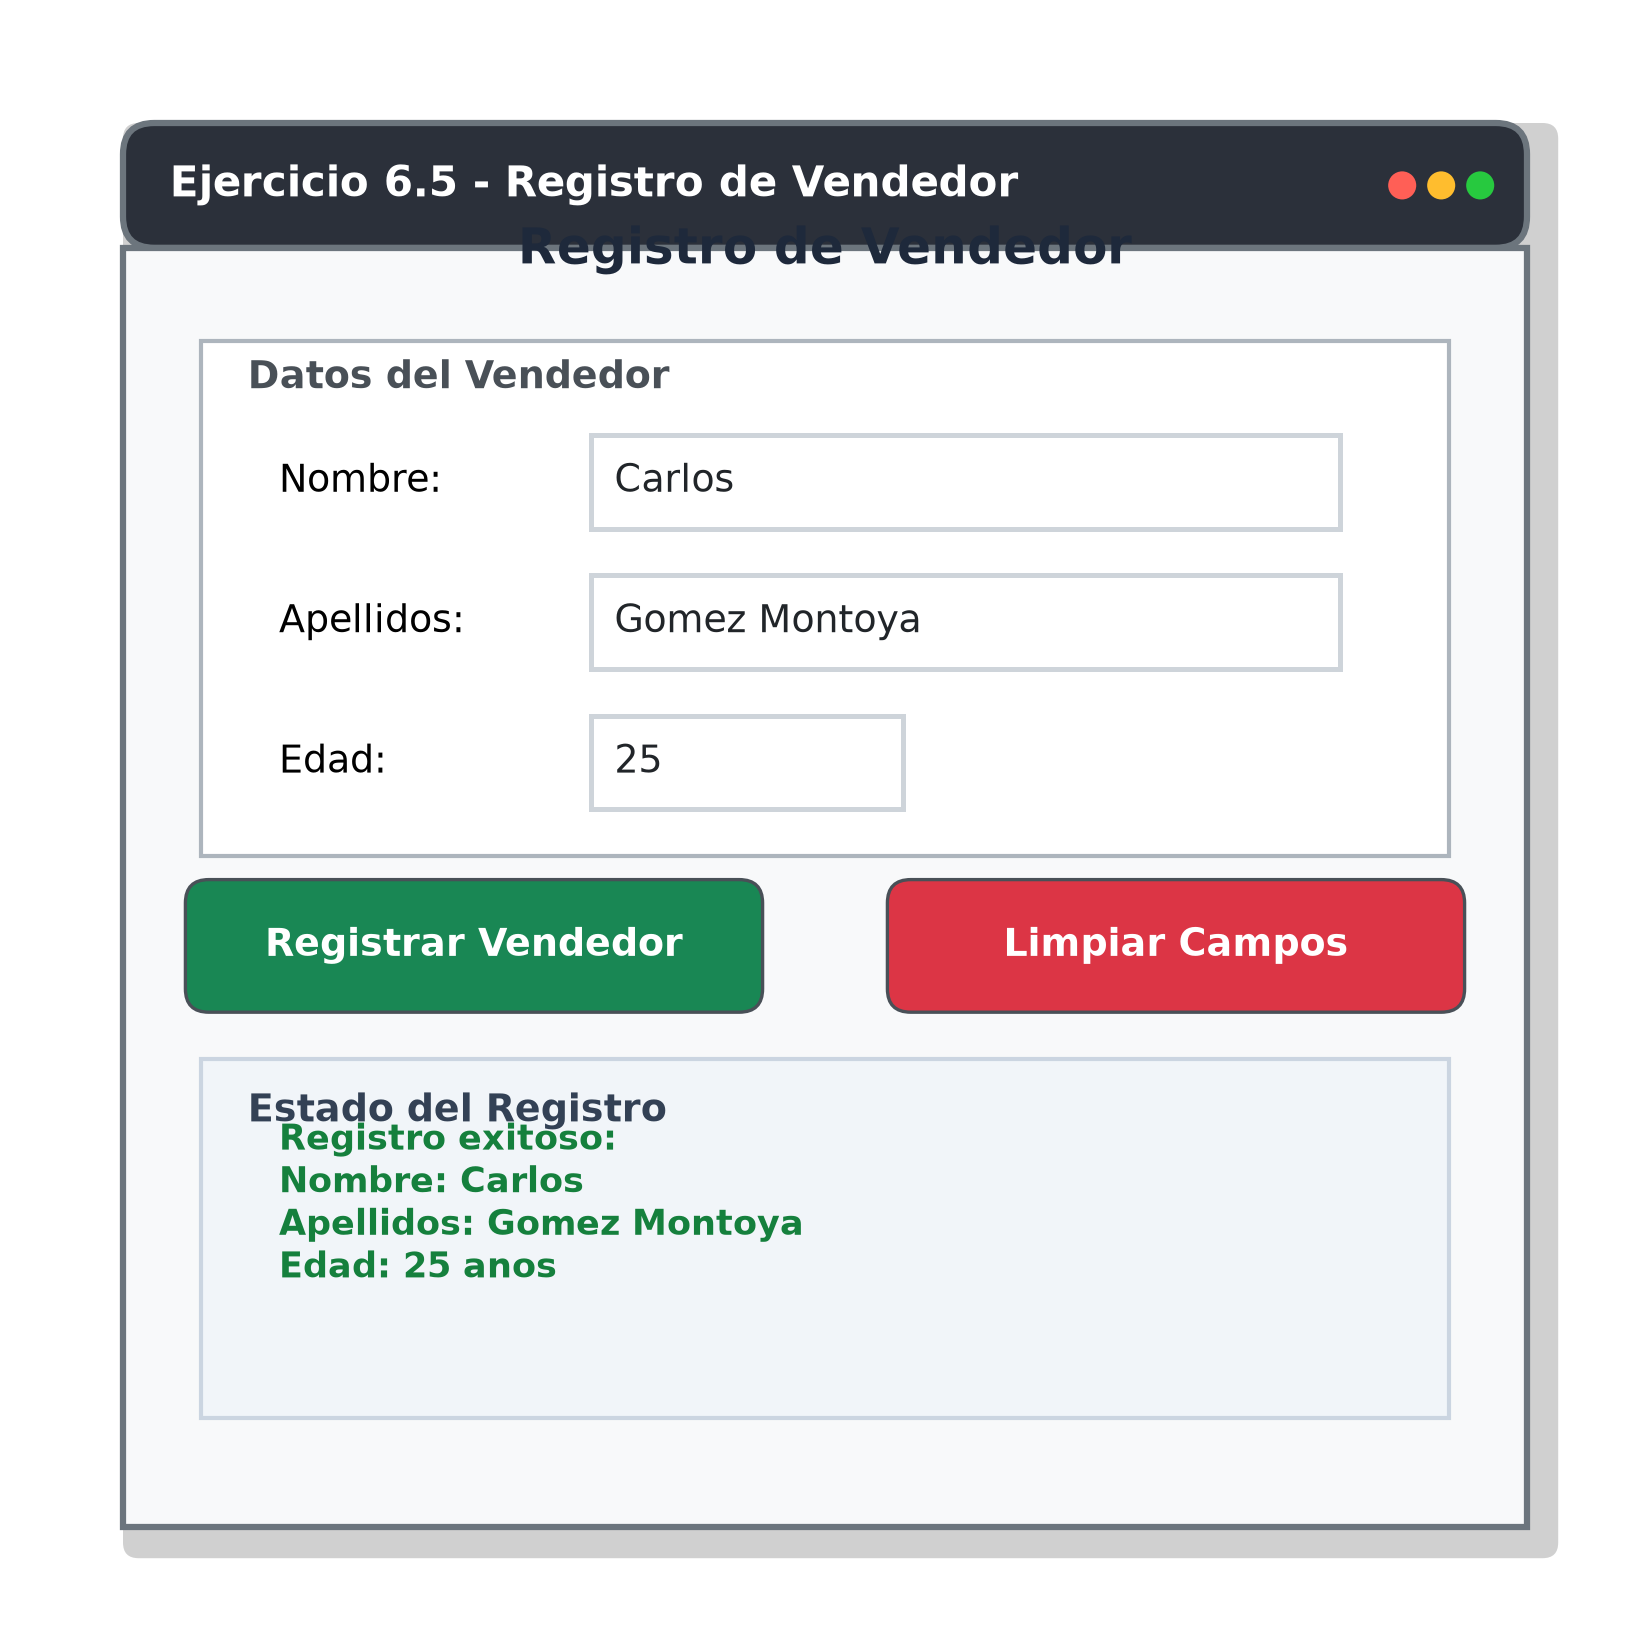
\includegraphics[width=0.52\textwidth]{figuras/ui_ejercicio6_5.png}
    \caption{Interfaz de usuario para el ejercicio 6.5 (Página 406).}
    \label{fig:ui_65}
\end{figure}

\subsection{Diagramas UML}

\subsubsection{Diagrama de clases}
En la figura \ref{fig:clases_65} se detalla el diagrama de clases del ejercicio. La clase \texttt{Vendedor} contiene la lógica de negocio y validación estricta de datos, mientras que la clase \texttt{VentanaVendedor} gestiona los componentes visuales e interactúa con la clase de dominio.

\begin{figure}[H]
    \centering
    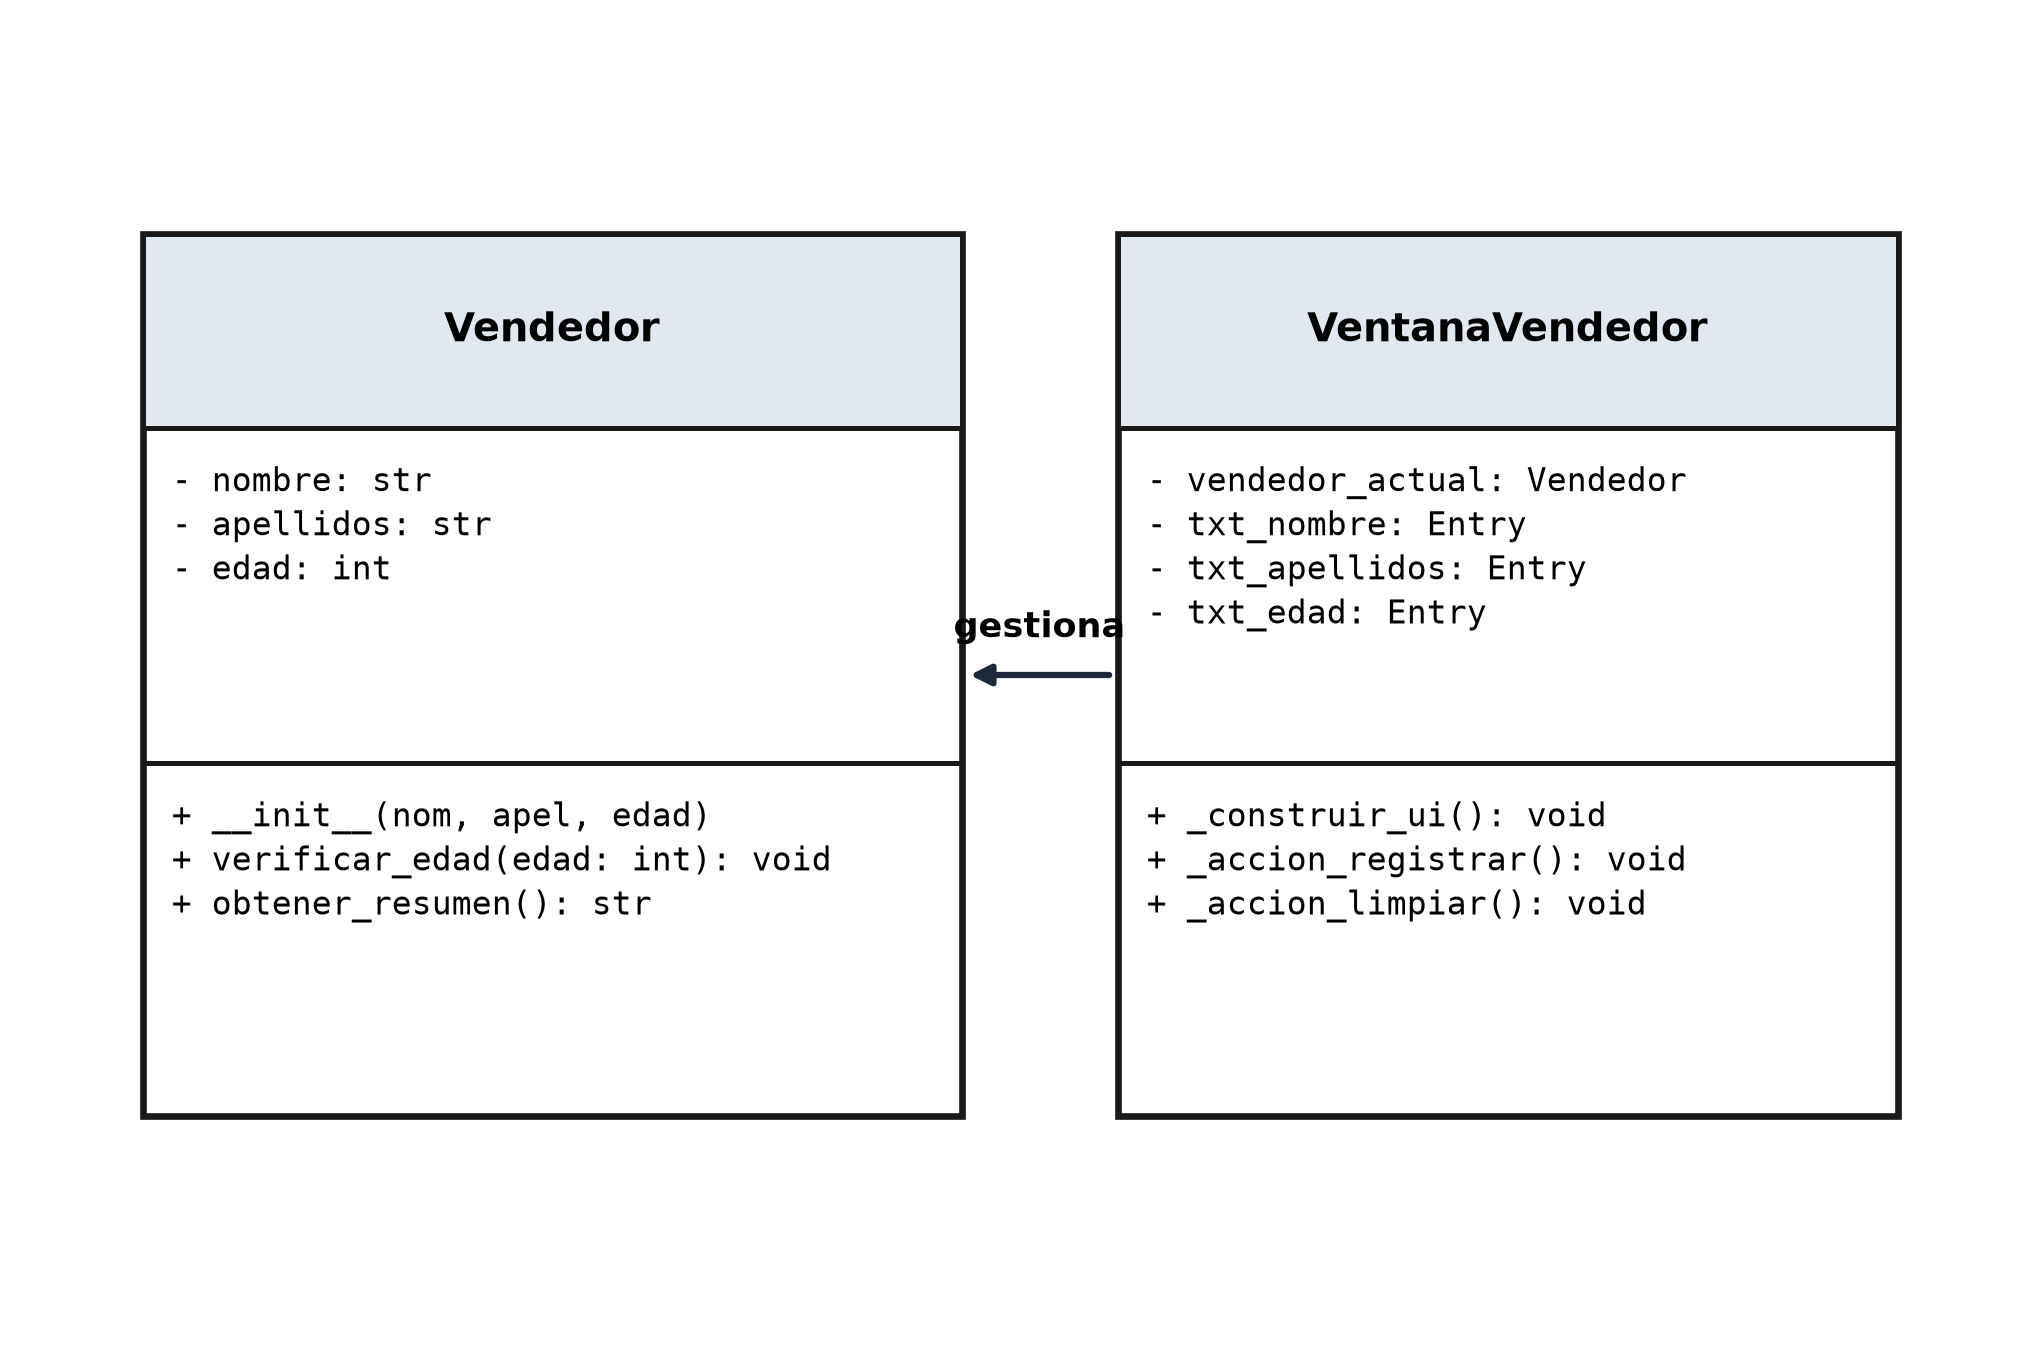
\includegraphics[width=0.78\textwidth]{figuras/clases_ejercicio6_5.png}
    \caption{Diagrama de clases para el ejercicio 6.5.}
    \label{fig:clases_65}
\end{figure}

\subsubsection{Casos de uso}
La figura \ref{fig:casos_65} representa las acciones ejecutables en el módulo de registro de vendedores.

\begin{figure}[H]
    \centering
    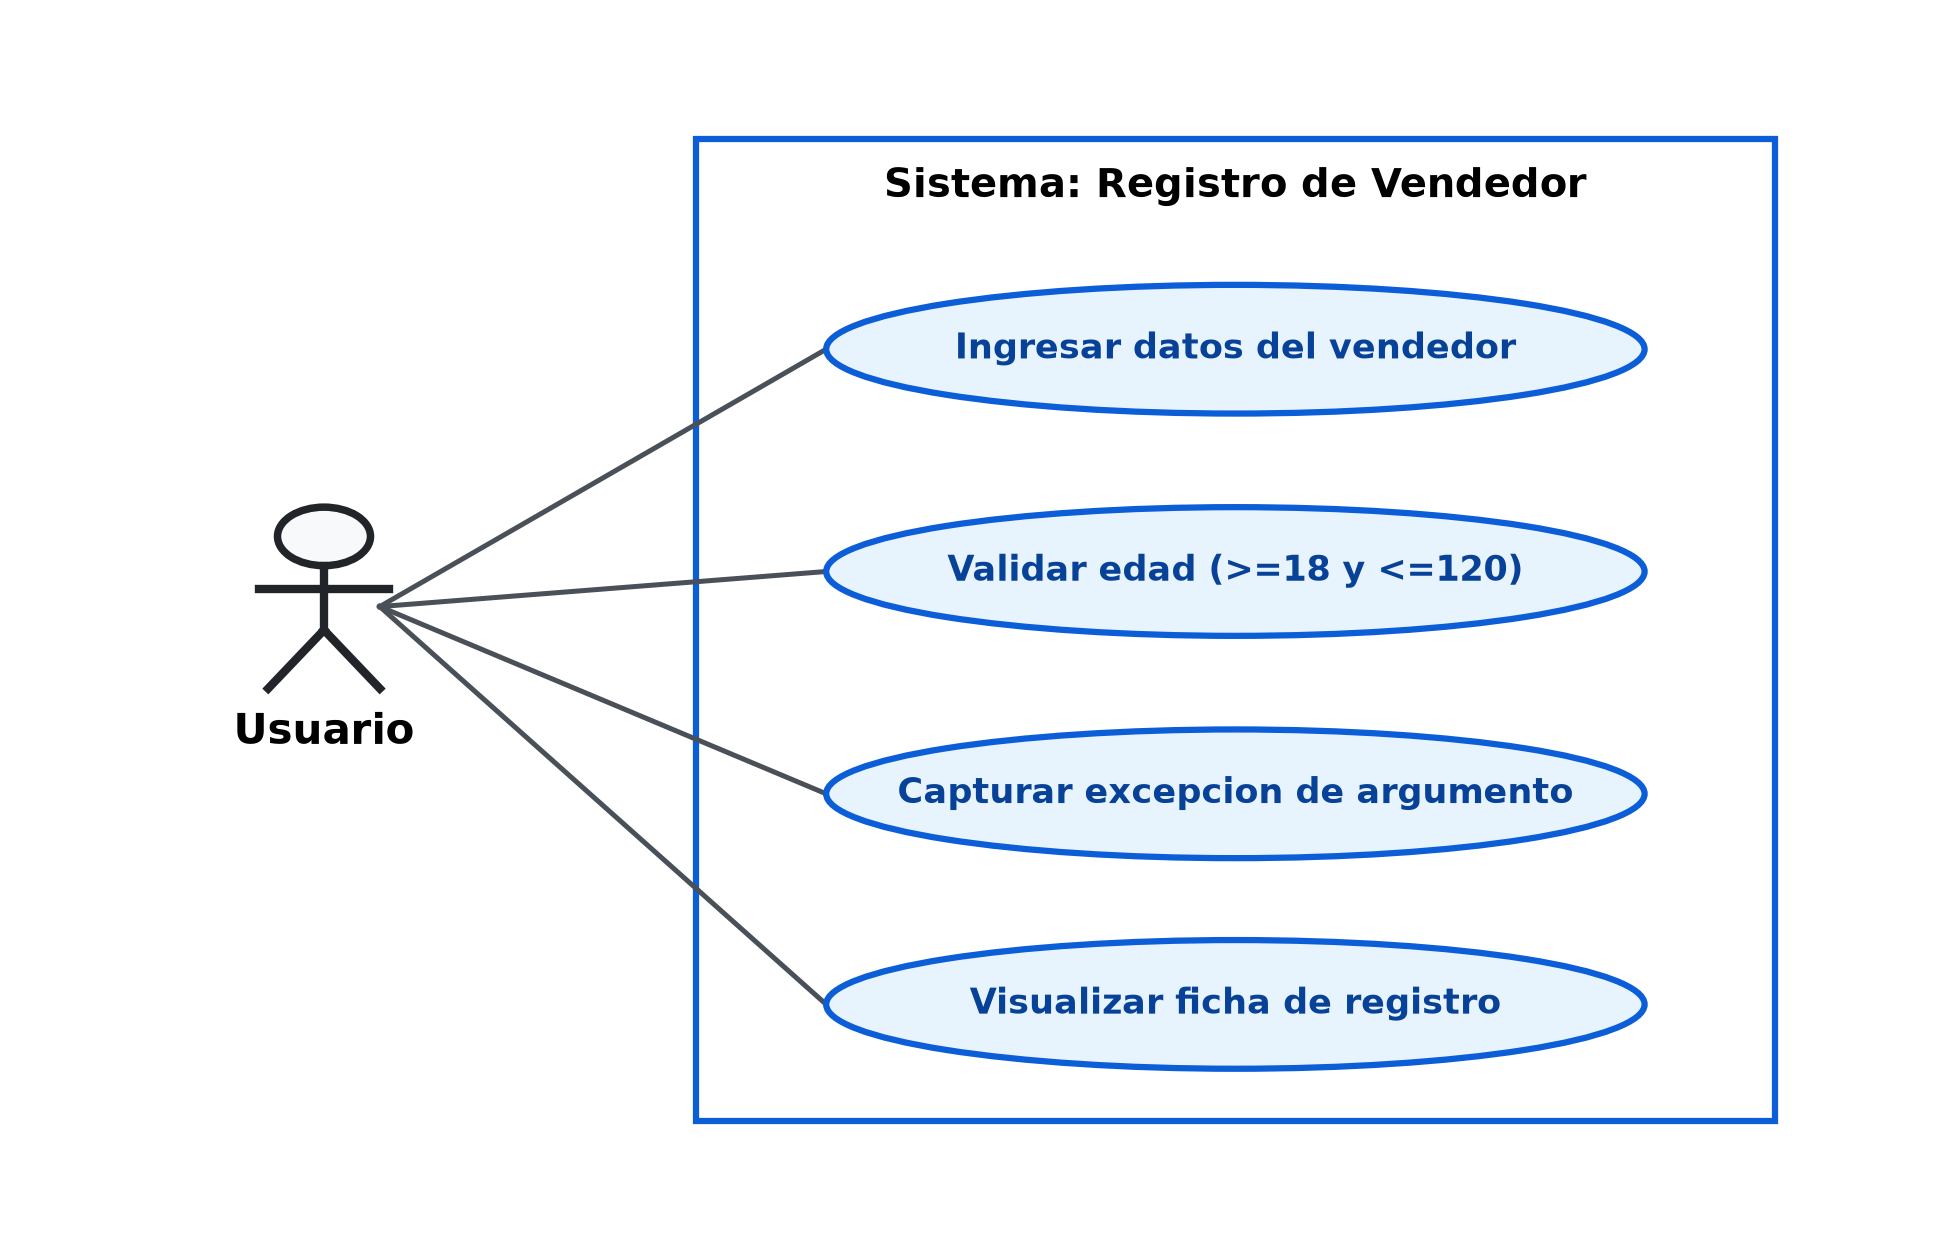
\includegraphics[width=0.75\textwidth]{figuras/casos_ejercicio6_5.png}
    \caption{Diagrama de casos de uso para el ejercicio 6.5.}
    \label{fig:casos_65}
\end{figure}

\begin{itemize}
    \item \textbf{Ingresar datos del vendedor:} captura los datos personales del usuario.
    \item \textbf{Validar edad ($\ge 18$ y $\le 120$):} el sistema evalúa la restricción de mayoría de edad y el rango biológico admitido.
    \item \textbf{Capturar excepción de argumento:} intercepta cualquier violación de los datos antes de permitir la persistencia en memoria.
    \item \textbf{Visualizar ficha de registro:} presenta los atributos del vendedor en el panel de resultados.
\end{itemize}

\clearpage

% ==============================================================================
% EJERCICIO 3
% ==============================================================================
\section{Ejercicio Página 412 (Ejercicio 6.6: Catchs múltiples)}

\noindent\textbf{Enlace a GitHub:} \\
\url{https://github.com/yguzmanm-sys/POO-2026-2S/blob/main/Actividad4/Ejercicio6_6.py}

\subsection{Descripción del Problema}
El ejercicio 6.6 del texto guía presenta el uso de múltiples bloques \texttt{catch} asociados a un único bloque \texttt{try}. Esto permite discriminar con precisión la naturaleza del error ocurrido en operaciones matemáticas, distinguiendo entre errores de formato de datos (\texttt{InputMismatchException} o \texttt{ValueError}) y errores de cálculo matemático (\texttt{ArithmeticException} o \texttt{ArithmeticError}), tales como el cálculo del logaritmo neperiano de números negativos o menores o iguales a cero, y la raíz cuadrada de valores negativos.

\subsection{Código Fuente}

\begin{lstlisting}[language=Python, caption=Cálculos numéricos con catchs múltiples en Python, label=lst:ej66]
import math
import tkinter as tk
from tkinter import ttk, messagebox

class CalculosNumericos:
    @staticmethod
    def calcular_logaritmo(valor: float) -> float:
        if valor <= 0:
            raise ArithmeticError("El valor debe ser un numero positivo mayor a cero para calcular el logaritmo neperiano.")
        return math.log(valor)

    @staticmethod
    def calcular_raiz(valor: float) -> float:
        if valor < 0:
            raise ArithmeticError("El valor debe ser un numero no negativo para calcular la raiz cuadrada.")
        return math.sqrt(valor)


class VentanaCalculos(tk.Tk):
    def __init__(self):
        super().__init__()
        self.title("Ejercicio 6.6 - Calculos Numericos y Catchs Multiples")
        self.geometry("460x380")
        self.resizable(False, False)
        self._construir_ui()

    def _construir_ui(self):
        marco = ttk.Frame(self, padding="20")
        marco.pack(fill=tk.BOTH, expand=True)

        lbl_titulo = ttk.Label(marco, text="Calculos Numericos y Excepciones Multiples", font=("Segoe UI", 12, "bold"))
        lbl_titulo.pack(pady=(0, 15))

        marco_entrada = ttk.LabelFrame(marco, text="Entrada de Datos", padding="12")
        marco_entrada.pack(fill=tk.X, pady=5)

        ttk.Label(marco_entrada, text="Ingrese un valor numerico:").grid(row=0, column=0, sticky=tk.W, pady=4)
        self.txt_valor = ttk.Entry(marco_entrada, width=18)
        self.txt_valor.grid(row=0, column=1, sticky=tk.W, padx=8, pady=4)

        marco_botones = ttk.Frame(marco)
        marco_botones.pack(fill=tk.X, pady=12)

        btn_log = ttk.Button(marco_botones, text="Logaritmo Neperiano", command=self._accion_logaritmo)
        btn_log.pack(side=tk.LEFT, padx=4)

        btn_raiz = ttk.Button(marco_botones, text="Raiz Cuadrada", command=self._accion_raiz)
        btn_raiz.pack(side=tk.LEFT, padx=4)

        btn_limpiar = ttk.Button(marco_botones, text="Limpiar", command=self._accion_limpiar)
        btn_limpiar.pack(side=tk.LEFT, padx=4)

        self.marco_salida = ttk.LabelFrame(marco, text="Resultado y Captura de Excepciones", padding="12")
        self.marco_salida.pack(fill=tk.BOTH, expand=True, pady=5)

        self.lbl_resultado = ttk.Label(self.marco_salida, text="Resultado = ", font=("Segoe UI", 10))
        self.lbl_resultado.pack(anchor=tk.W, pady=2)

        self.lbl_diagnostico = ttk.Label(self.marco_salida, text="Estado: En espera de operacion.", font=("Segoe UI", 9), foreground="gray")
        self.lbl_diagnostico.pack(anchor=tk.W, pady=2)

    def _obtener_numero(self) -> float:
        texto = self.txt_valor.get().strip()
        if not texto:
            raise ValueError("El campo de valor se encuentra vacio.")
        try:
            return float(texto)
        except ValueError as e:
            raise ValueError("El dato ingresado no es numerico.") from e

    def _accion_logaritmo(self):
        try:
            val = self._obtener_numero()
            res = CalculosNumericos.calcular_logaritmo(val)
            self.lbl_resultado.config(text=f"Resultado = {res:.6f}")
            self.lbl_diagnostico.config(text="Operacion exitosa sin excepciones.", foreground="green")
        except ValueError as e:
            self.lbl_resultado.config(text="Resultado = Error")
            self.lbl_diagnostico.config(text=f"Catch ValueError: {e}", foreground="red")
            messagebox.showerror("Error de Formato", str(e))
        except ArithmeticError as e:
            self.lbl_resultado.config(text="Resultado = Error")
            self.lbl_diagnostico.config(text=f"Catch ArithmeticError: {e}", foreground="red")
            messagebox.showerror("Error Matematico", str(e))
        except Exception as e:
            self.lbl_resultado.config(text="Resultado = Error")
            self.lbl_diagnostico.config(text=f"Catch Exception: {e}", foreground="red")
            messagebox.showerror("Error Desconocido", str(e))

    def _accion_raiz(self):
        try:
            val = self._obtener_numero()
            res = CalculosNumericos.calcular_raiz(val)
            self.lbl_resultado.config(text=f"Resultado = {res:.6f}")
            self.lbl_diagnostico.config(text="Operacion exitosa sin excepciones.", foreground="green")
        except ValueError as e:
            self.lbl_resultado.config(text="Resultado = Error")
            self.lbl_diagnostico.config(text=f"Catch ValueError: {e}", foreground="red")
            messagebox.showerror("Error de Formato", str(e))
        except ArithmeticError as e:
            self.lbl_resultado.config(text="Resultado = Error")
            self.lbl_diagnostico.config(text=f"Catch ArithmeticError: {e}", foreground="red")
            messagebox.showerror("Error Matematico", str(e))
        except Exception as e:
            self.lbl_resultado.config(text="Resultado = Error")
            self.lbl_diagnostico.config(text=f"Catch Exception: {e}", foreground="red")
            messagebox.showerror("Error Desconocido", str(e))

    def _accion_limpiar(self):
        self.txt_valor.delete(0, tk.END)
        self.lbl_resultado.config(text="Resultado = ")
        self.lbl_diagnostico.config(text="Estado: En espera de operacion.", foreground="gray")


if __name__ == "__main__":
    app = VentanaCalculos()
    app.mainloop()
\end{lstlisting}

\subsection{Interfaz de usuario}
La figura \ref{fig:ui_66} presenta la interfaz gráfica para cálculos numéricos. Incluye una caja de texto para el operando numérico, botones dedicados para calcular el logaritmo neperiano y la raíz cuadrada, y una sección de diagnóstico donde se muestra el valor calculado o el tipo exacto de excepción capturada por la aplicación.

\begin{figure}[H]
    \centering
    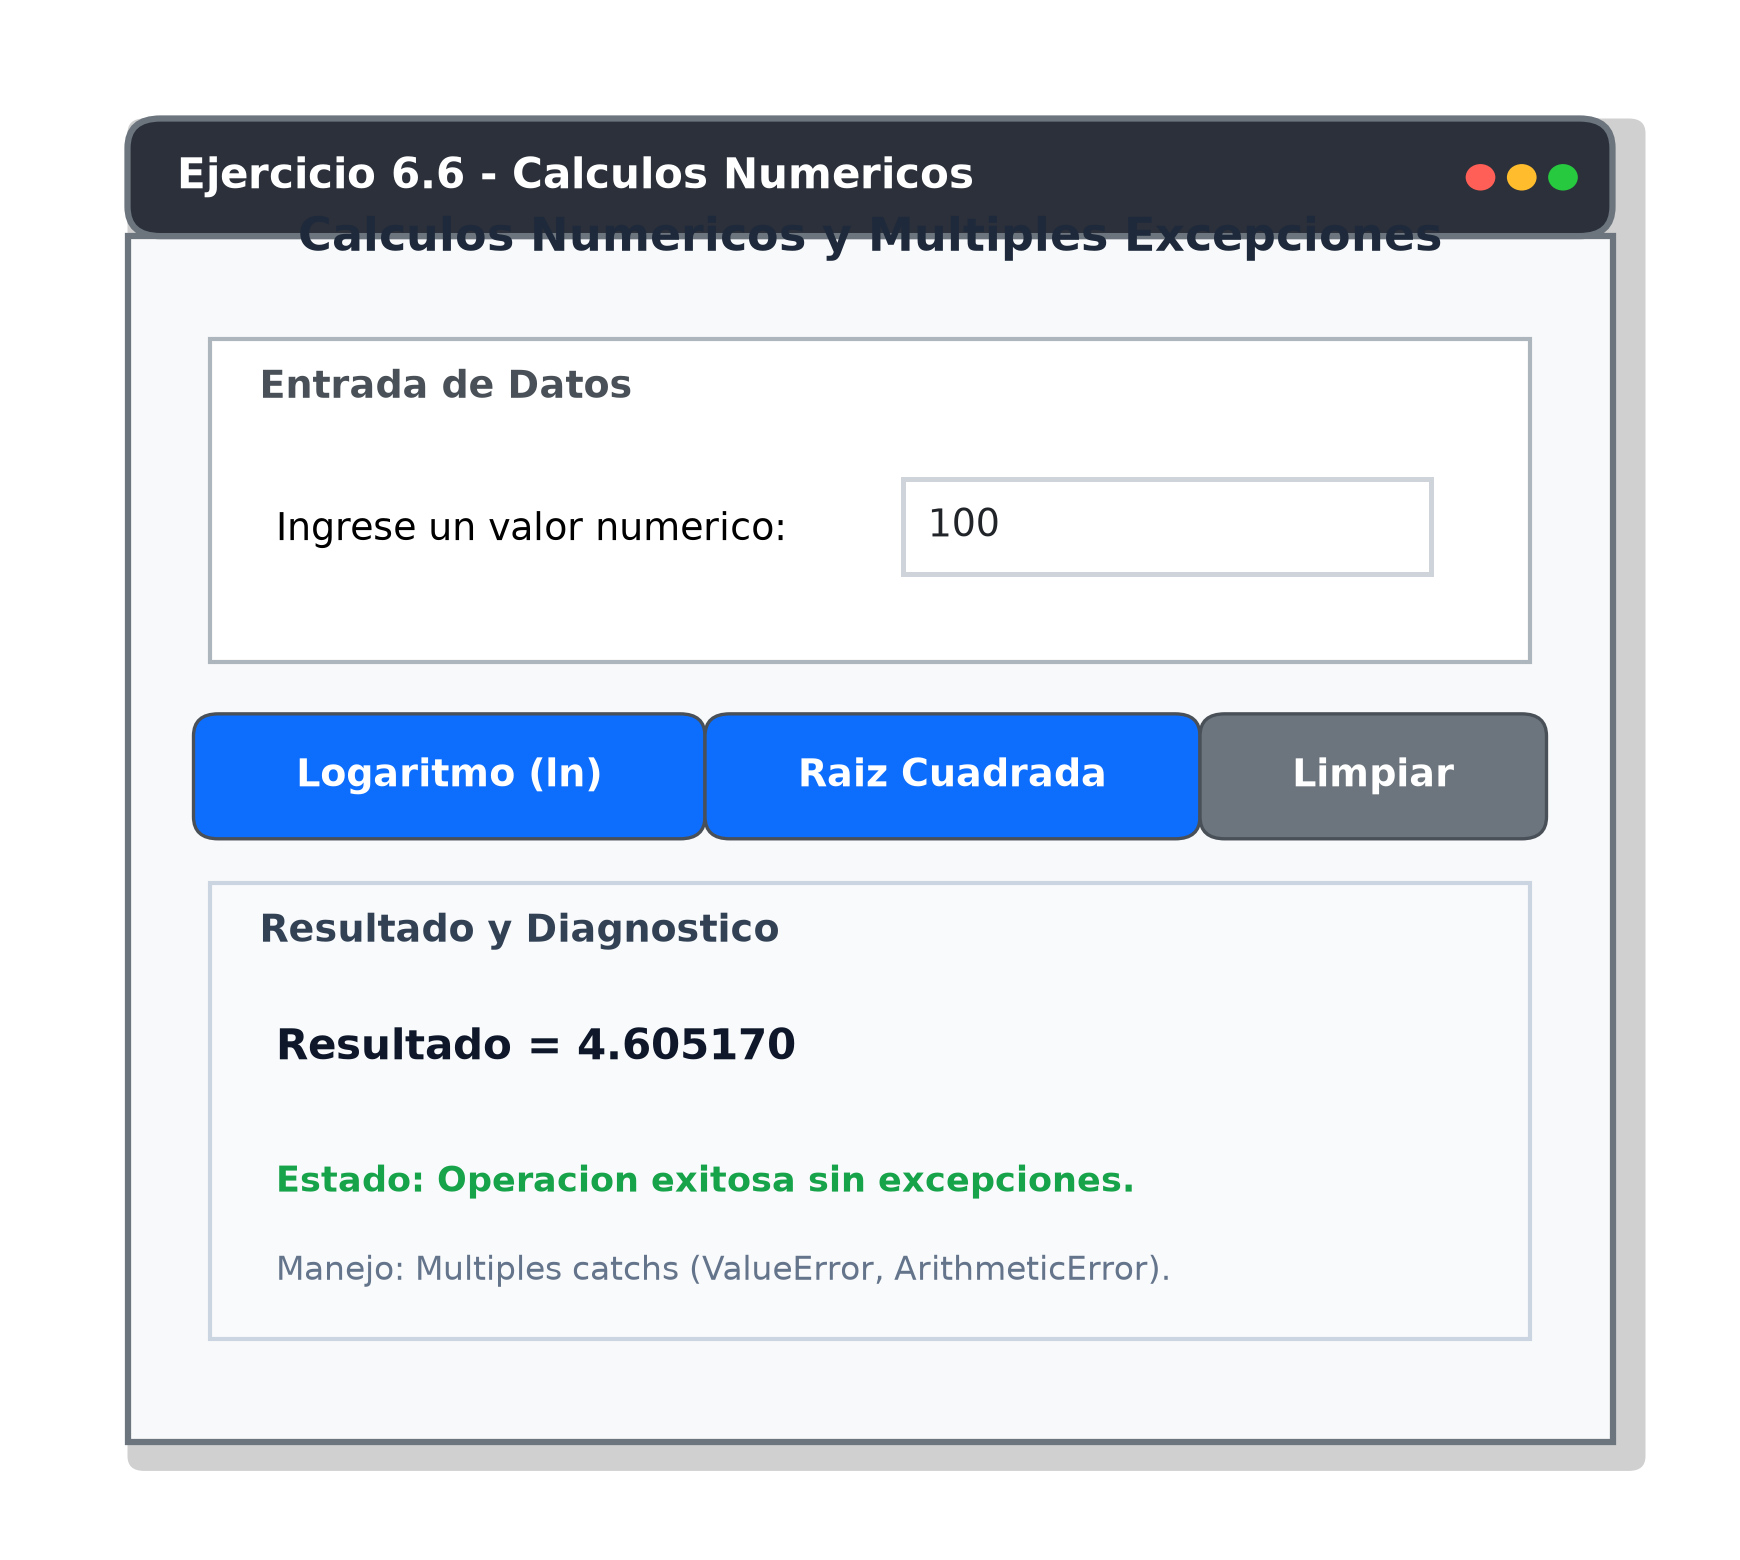
\includegraphics[width=0.55\textwidth]{figuras/ui_ejercicio6_6.png}
    \caption{Interfaz de usuario para el ejercicio 6.6 (Página 412).}
    \label{fig:ui_66}
\end{figure}

\subsection{Diagramas UML}

\subsubsection{Diagrama de clases}
En la figura \ref{fig:clases_66} se presenta el diagrama de clases del ejercicio 6.6. La clase \texttt{CalculosNumericos} proporciona métodos estáticos para las funciones matemáticas con validación estricta de precondiciones, mientras que la clase \texttt{VentanaCalculos} gestiona los eventos del usuario e implementa los bloques \texttt{catch} jerárquicos.

\begin{figure}[H]
    \centering
    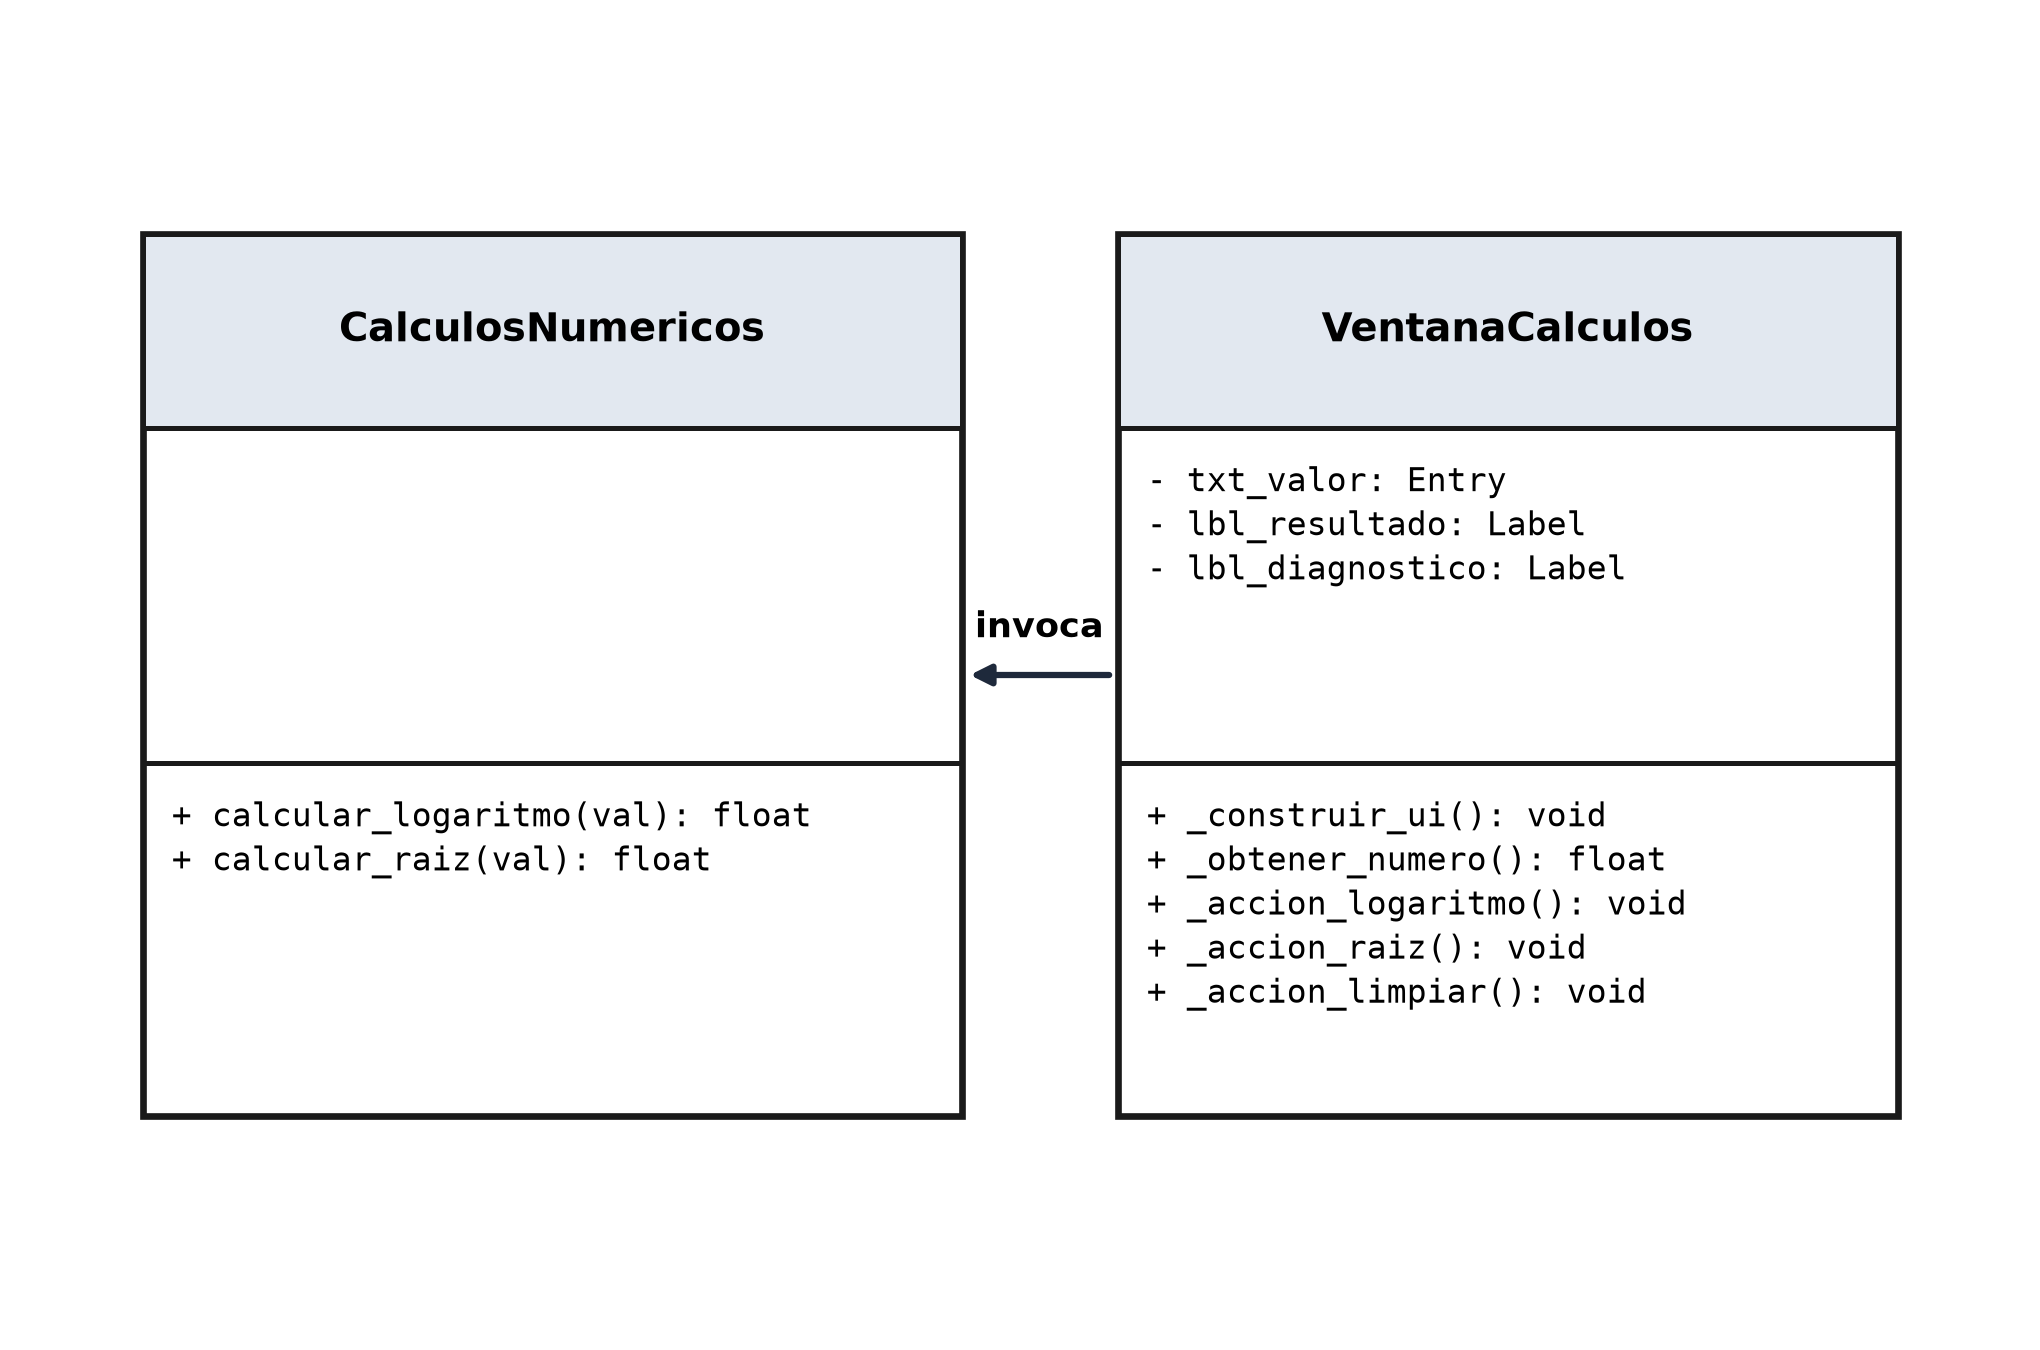
\includegraphics[width=0.78\textwidth]{figuras/clases_ejercicio6_6.png}
    \caption{Diagrama de clases para el ejercicio 6.6.}
    \label{fig:clases_66}
\end{figure}

\subsubsection{Casos de uso}
La figura \ref{fig:casos_66} ilustra el modelo de casos de uso para las operaciones numéricas.

\begin{figure}[H]
    \centering
    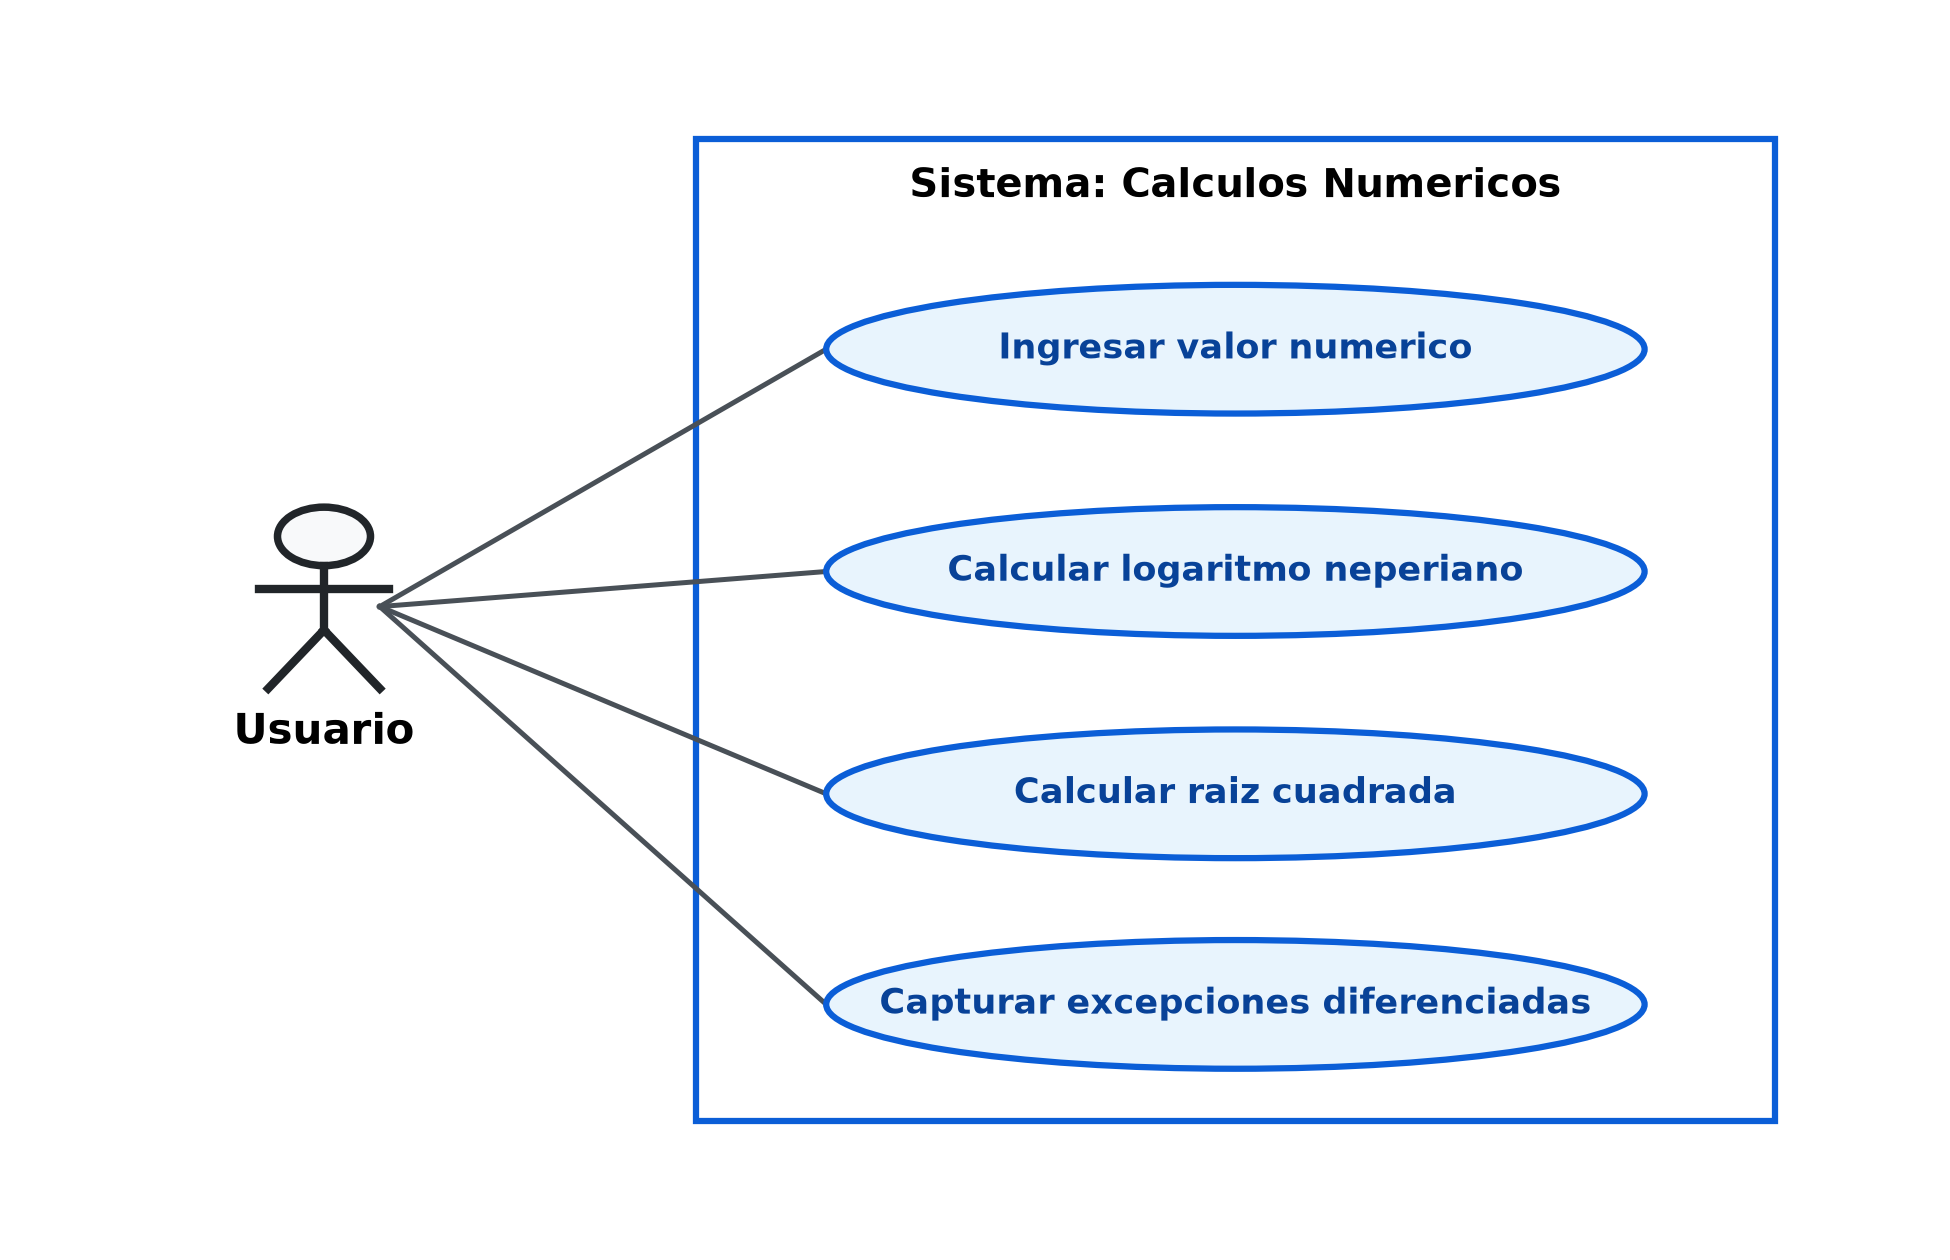
\includegraphics[width=0.75\textwidth]{figuras/casos_ejercicio6_6.png}
    \caption{Diagrama de casos de uso para el ejercicio 6.6.}
    \label{fig:casos_66}
\end{figure}

\begin{itemize}
    \item \textbf{Ingresar valor numérico:} suministra la entrada matemática.
    \item \textbf{Calcular logaritmo neperiano:} evalúa $\ln(x)$ validando que $x > 0$.
    \item \textbf{Calcular raíz cuadrada:} evalúa $\sqrt{x}$ validando que $x \ge 0$.
    \item \textbf{Capturar excepciones diferenciadas:} gestiona de forma individualizada los errores de sintaxis y los de dominio aritmético.
\end{itemize}

\clearpage

% ==============================================================================
% EJERCICIO 4
% ==============================================================================
\section{Ejercicio Página 418 (Ejercicio 6.7: Validación de campos)}

\noindent\textbf{Enlace a GitHub:} \\
\url{https://github.com/yguzmanm-sys/POO-2026-2S/blob/main/Actividad4/Ejercicio6_7.py}

\subsection{Descripción del Problema}
El ejercicio 6.7 del texto guía ilustra cómo las excepciones son una herramienta fundamental para la validación de formularios y la integridad de colecciones. Se modela un equipo de maratón de programación conformado por hasta 3 programadores. Cada programador posee nombre y apellidos, los cuales deben contener exclusivamente caracteres alfabéticos, no superar los 20 caracteres de longitud y no ser vacíos. Además, el equipo posee un límite estricto de cupo: si se intenta registrar un cuarto integrante, se debe disparar una excepción de capacidad excedida.

\subsection{Código Fuente}

\begin{lstlisting}[language=Python, caption=Validación de campos y equipo de maratón en Python, label=lst:ej67]
import tkinter as tk
from tkinter import ttk, messagebox

class Programador:
    def __init__(self, nombre: str, apellidos: str):
        self.nombre = self._validar_campo(nombre, "Nombre")
        self.apellidos = self._validar_campo(apellidos, "Apellidos")

    @staticmethod
    def _validar_campo(valor: str, nombre_campo: str) -> str:
        limpio = valor.strip()
        if not limpio:
            raise ValueError(f"El campo '{nombre_campo}' no puede estar vacio.")
        if len(limpio) > 20:
            raise ValueError(f"La longitud de '{nombre_campo}' no debe ser superior a 20 caracteres.")
        if any(char.isdigit() for char in limpio):
            raise ValueError(f"El campo '{nombre_campo}' no puede contener caracteres numericos.")
        return limpio


class EquipoMaratonProgramacion:
    CAPACIDAD_MAXIMA = 3

    def __init__(self, nombre_equipo: str, universidad: str, lenguaje: str):
        if not nombre_equipo.strip():
            raise ValueError("El nombre del equipo no puede estar vacio.")
        if not universidad.strip():
            raise ValueError("El nombre de la universidad no puede estar vacio.")
        if not lenguaje.strip():
            raise ValueError("El lenguaje de programacion no puede estar vacio.")
        if len(nombre_equipo.strip()) > 20:
            raise ValueError("El nombre del equipo no debe superar 20 caracteres.")
        if len(universidad.strip()) > 20:
            raise ValueError("La universidad no debe superar 20 caracteres.")
        if len(lenguaje.strip()) > 20:
            raise ValueError("El lenguaje no debe superar 20 caracteres.")

        self.nombre_equipo = nombre_equipo.strip()
        self.universidad = universidad.strip()
        self.lenguaje = lenguaje.strip()
        self.programadores: list[Programador] = []

    def esta_lleno(self) -> bool:
        return len(self.programadores) >= self.CAPACIDAD_MAXIMA

    def anadir_programador(self, programador: Programador):
        if self.esta_lleno():
            raise OverflowError("El equipo de programacion esta completo (maximo 3 integrantes).")
        self.programadores.append(programador)


class VentanaEquipoMaraton(tk.Tk):
    def __init__(self):
        super().__init__()
        self.title("Ejercicio 6.7 - Equipo de Maraton de Programacion")
        self.geometry("540x550")
        self.resizable(False, False)
        self.equipo = None
        self._construir_ui()

    def _construir_ui(self):
        marco = ttk.Frame(self, padding="15")
        marco.pack(fill=tk.BOTH, expand=True)

        lbl_titulo = ttk.Label(marco, text="Registro y Validacion de Equipo", font=("Segoe UI", 13, "bold"))
        lbl_titulo.pack(pady=(0, 10))

        marco_equipo = ttk.LabelFrame(marco, text="Datos del Equipo", padding="10")
        marco_equipo.pack(fill=tk.X, pady=5)

        ttk.Label(marco_equipo, text="Nombre Equipo:").grid(row=0, column=0, sticky=tk.W, pady=3)
        self.txt_nombre_eq = ttk.Entry(marco_equipo, width=22)
        self.txt_nombre_eq.grid(row=0, column=1, padx=5, pady=3)

        ttk.Label(marco_equipo, text="Universidad:").grid(row=0, column=2, sticky=tk.W, padx=(10, 0), pady=3)
        self.txt_universidad = ttk.Entry(marco_equipo, width=22)
        self.txt_universidad.grid(row=0, column=3, padx=5, pady=3)

        ttk.Label(marco_equipo, text="Lenguaje:").grid(row=1, column=0, sticky=tk.W, pady=3)
        self.txt_lenguaje = ttk.Entry(marco_equipo, width=22)
        self.txt_lenguaje.grid(row=1, column=1, padx=5, pady=3)

        btn_crear_eq = ttk.Button(marco_equipo, text="Crear/Actualizar Equipo", command=self._accion_crear_equipo)
        btn_crear_eq.grid(row=1, column=2, columnspan=2, sticky=tk.EW, padx=5, pady=3)

        marco_prog = ttk.LabelFrame(marco, text="Anadir Programador (Max. 3)", padding="10")
        marco_prog.pack(fill=tk.X, pady=8)

        ttk.Label(marco_prog, text="Nombre:").grid(row=0, column=0, sticky=tk.W, pady=3)
        self.txt_prog_nombre = ttk.Entry(marco_prog, width=22)
        self.txt_prog_nombre.grid(row=0, column=1, padx=5, pady=3)

        ttk.Label(marco_prog, text="Apellidos:").grid(row=0, column=2, sticky=tk.W, padx=(10, 0), pady=3)
        self.txt_prog_apellidos = ttk.Entry(marco_prog, width=22)
        self.txt_prog_apellidos.grid(row=0, column=3, padx=5, pady=3)

        marco_btn_prog = ttk.Frame(marco_prog)
        marco_btn_prog.grid(row=1, column=0, columnspan=4, pady=(8, 2))

        btn_anadir = ttk.Button(marco_btn_prog, text="Anadir Programador", command=self._accion_anadir_prog)
        btn_anadir.pack(side=tk.LEFT, padx=5)

        btn_limpiar_p = ttk.Button(marco_btn_prog, text="Limpiar Campos", command=self._accion_limpiar_campos)
        btn_limpiar_p.pack(side=tk.LEFT, padx=5)

        btn_reiniciar = ttk.Button(marco_btn_prog, text="Reiniciar Todo", command=self._accion_reiniciar)
        btn_reiniciar.pack(side=tk.LEFT, padx=5)

        marco_lista = ttk.LabelFrame(marco, text="Programadores Inscritos", padding="10")
        marco_lista.pack(fill=tk.BOTH, expand=True, pady=5)

        self.lbl_conteo = ttk.Label(marco_lista, text="Integrantes registrados: 0 / 3", font=("Segoe UI", 9, "bold"))
        self.lbl_conteo.pack(anchor=tk.W, pady=(0, 5))

        columnas = ("num", "nombre", "apellidos")
        self.tabla = ttk.Treeview(marco_lista, columns=columnas, show="headings", height=4)
        self.tabla.heading("num", text="#")
        self.tabla.heading("nombre", text="Nombre")
        self.tabla.heading("apellidos", text="Apellidos")
        self.tabla.column("num", width=40, anchor=tk.CENTER)
        self.tabla.column("nombre", width=200)
        self.tabla.column("apellidos", width=200)
        self.tabla.pack(fill=tk.BOTH, expand=True)

    def _accion_crear_equipo(self):
        try:
            nom = self.txt_nombre_eq.get()
            uni = self.txt_universidad.get()
            leng = self.txt_lenguaje.get()
            self.equipo = EquipoMaratonProgramacion(nom, uni, leng)
            self._actualizar_tabla()
            messagebox.showinfo("Equipo Creado", f"Equipo '{nom}' inicializado correctamente.")
        except ValueError as e:
            messagebox.showerror("Error de Validacion", str(e))

    def _accion_anadir_prog(self):
        if not self.equipo:
            messagebox.showerror("Error", "Primero debe crear e inicializar los datos del equipo.")
            return

        try:
            nombre = self.txt_prog_nombre.get()
            apellidos = self.txt_prog_apellidos.get()
            nuevo_p = Programador(nombre, apellidos)
            self.equipo.anadir_programador(nuevo_p)
            self._actualizar_tabla()
            self.txt_prog_nombre.delete(0, tk.END)
            self.txt_prog_apellidos.delete(0, tk.END)
            messagebox.showinfo("Programador Anadido", "Integrante registrado con exito.")
        except (ValueError, OverflowError) as e:
            messagebox.showerror("Excepcion Capturada", str(e))

    def _actualizar_tabla(self):
        for item in self.tabla.get_children():
            self.tabla.delete(item)
        if self.equipo:
            for idx, p in enumerate(self.equipo.programadores, start=1):
                self.tabla.insert("", tk.END, values=(idx, p.nombre, p.apellidos))
            total = len(self.equipo.programadores)
            self.lbl_conteo.config(text=f"Integrantes registrados: {total} / {self.equipo.CAPACIDAD_MAXIMA}")
        else:
            self.lbl_conteo.config(text="Integrantes registrados: 0 / 3")

    def _accion_limpiar_campos(self):
        self.txt_prog_nombre.delete(0, tk.END)
        self.txt_prog_apellidos.delete(0, tk.END)

    def _accion_reiniciar(self):
        self.txt_nombre_eq.delete(0, tk.END)
        self.txt_universidad.delete(0, tk.END)
        self.txt_lenguaje.delete(0, tk.END)
        self.txt_prog_nombre.delete(0, tk.END)
        self.txt_prog_apellidos.delete(0, tk.END)
        self.equipo = None
        self._actualizar_tabla()


if __name__ == "__main__":
    app = VentanaEquipoMaraton()
    app.mainloop()
\end{lstlisting}

\subsection{Interfaz de usuario}
La figura \ref{fig:ui_67} muestra la aplicación de gestión del equipo de maratón. Permite ingresar y actualizar los datos del equipo, añadir programadores validando al instante las restricciones, y visualizar en una tabla (\texttt{Treeview}) el conteo en tiempo real de los integrantes registrados sobre la capacidad máxima.

\begin{figure}[H]
    \centering
    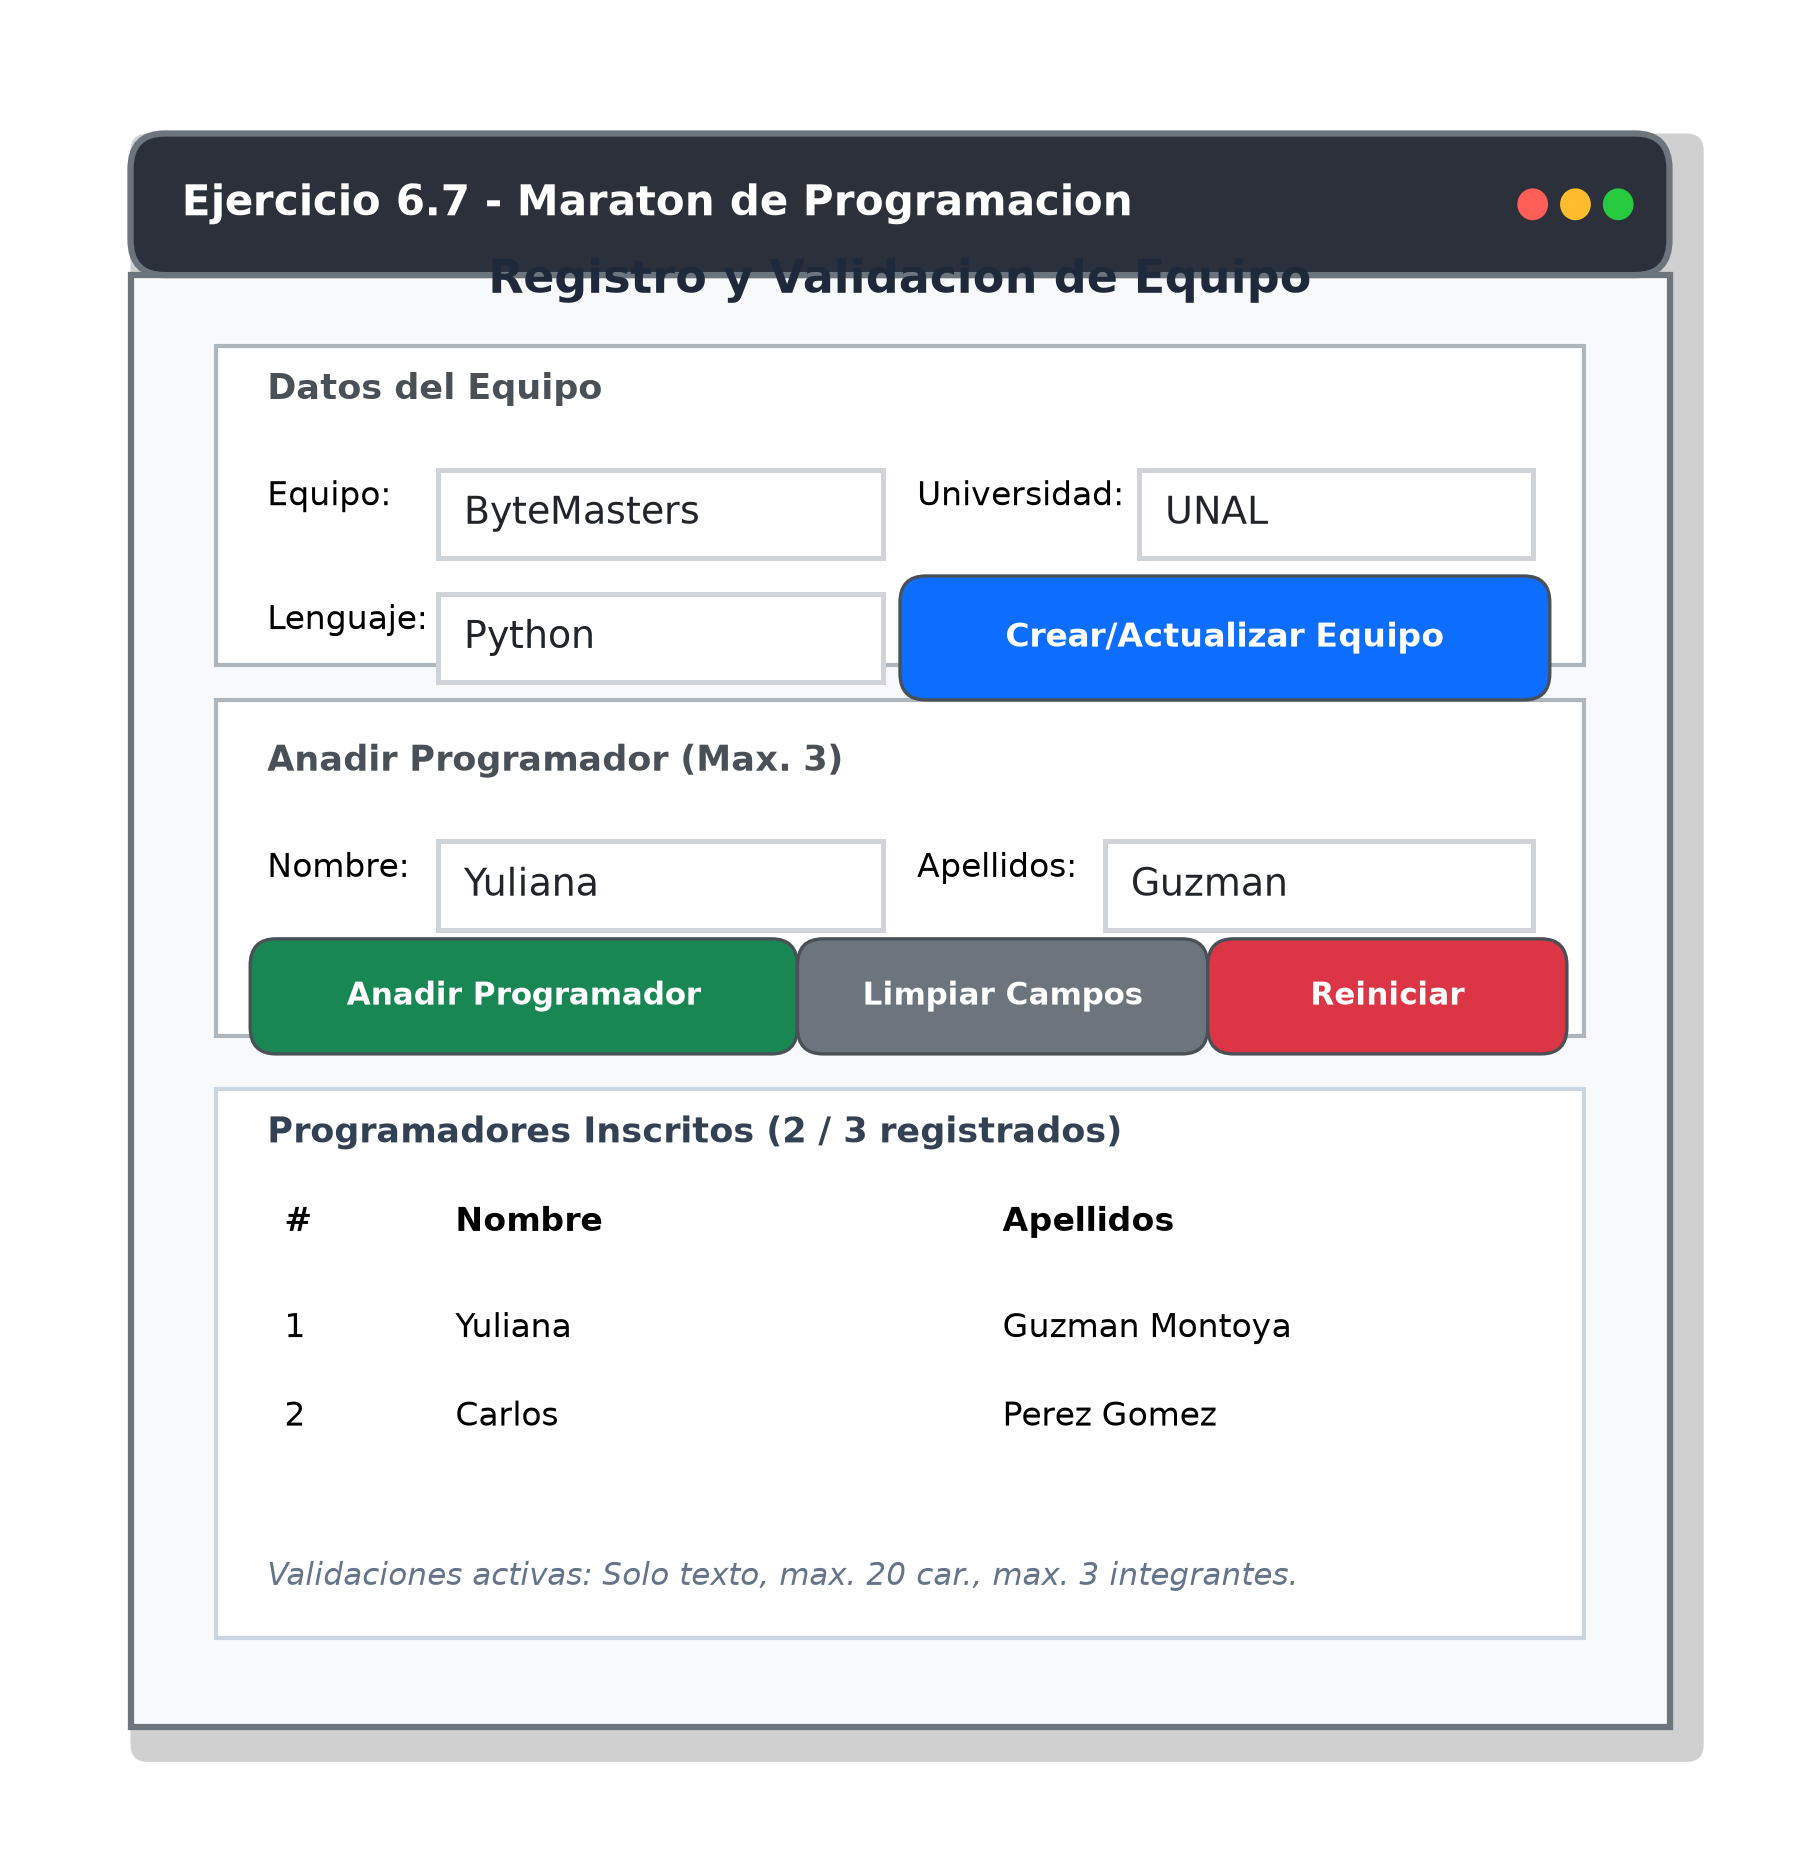
\includegraphics[width=0.55\textwidth]{figuras/ui_ejercicio6_7.png}
    \caption{Interfaz de usuario para el ejercicio 6.7 (Página 418).}
    \label{fig:ui_67}
\end{figure}

\subsection{Diagramas UML}

\subsubsection{Diagrama de clases}
La figura \ref{fig:clases_67} exhibe el diagrama de clases con la relación de composición estricta entre \texttt{EquipoMaratonProgramacion} y \texttt{Programador} (cardinalidad 1 a 3), y la interacción con la clase de interfaz \texttt{VentanaEquipoMaraton}.

\begin{figure}[H]
    \centering
    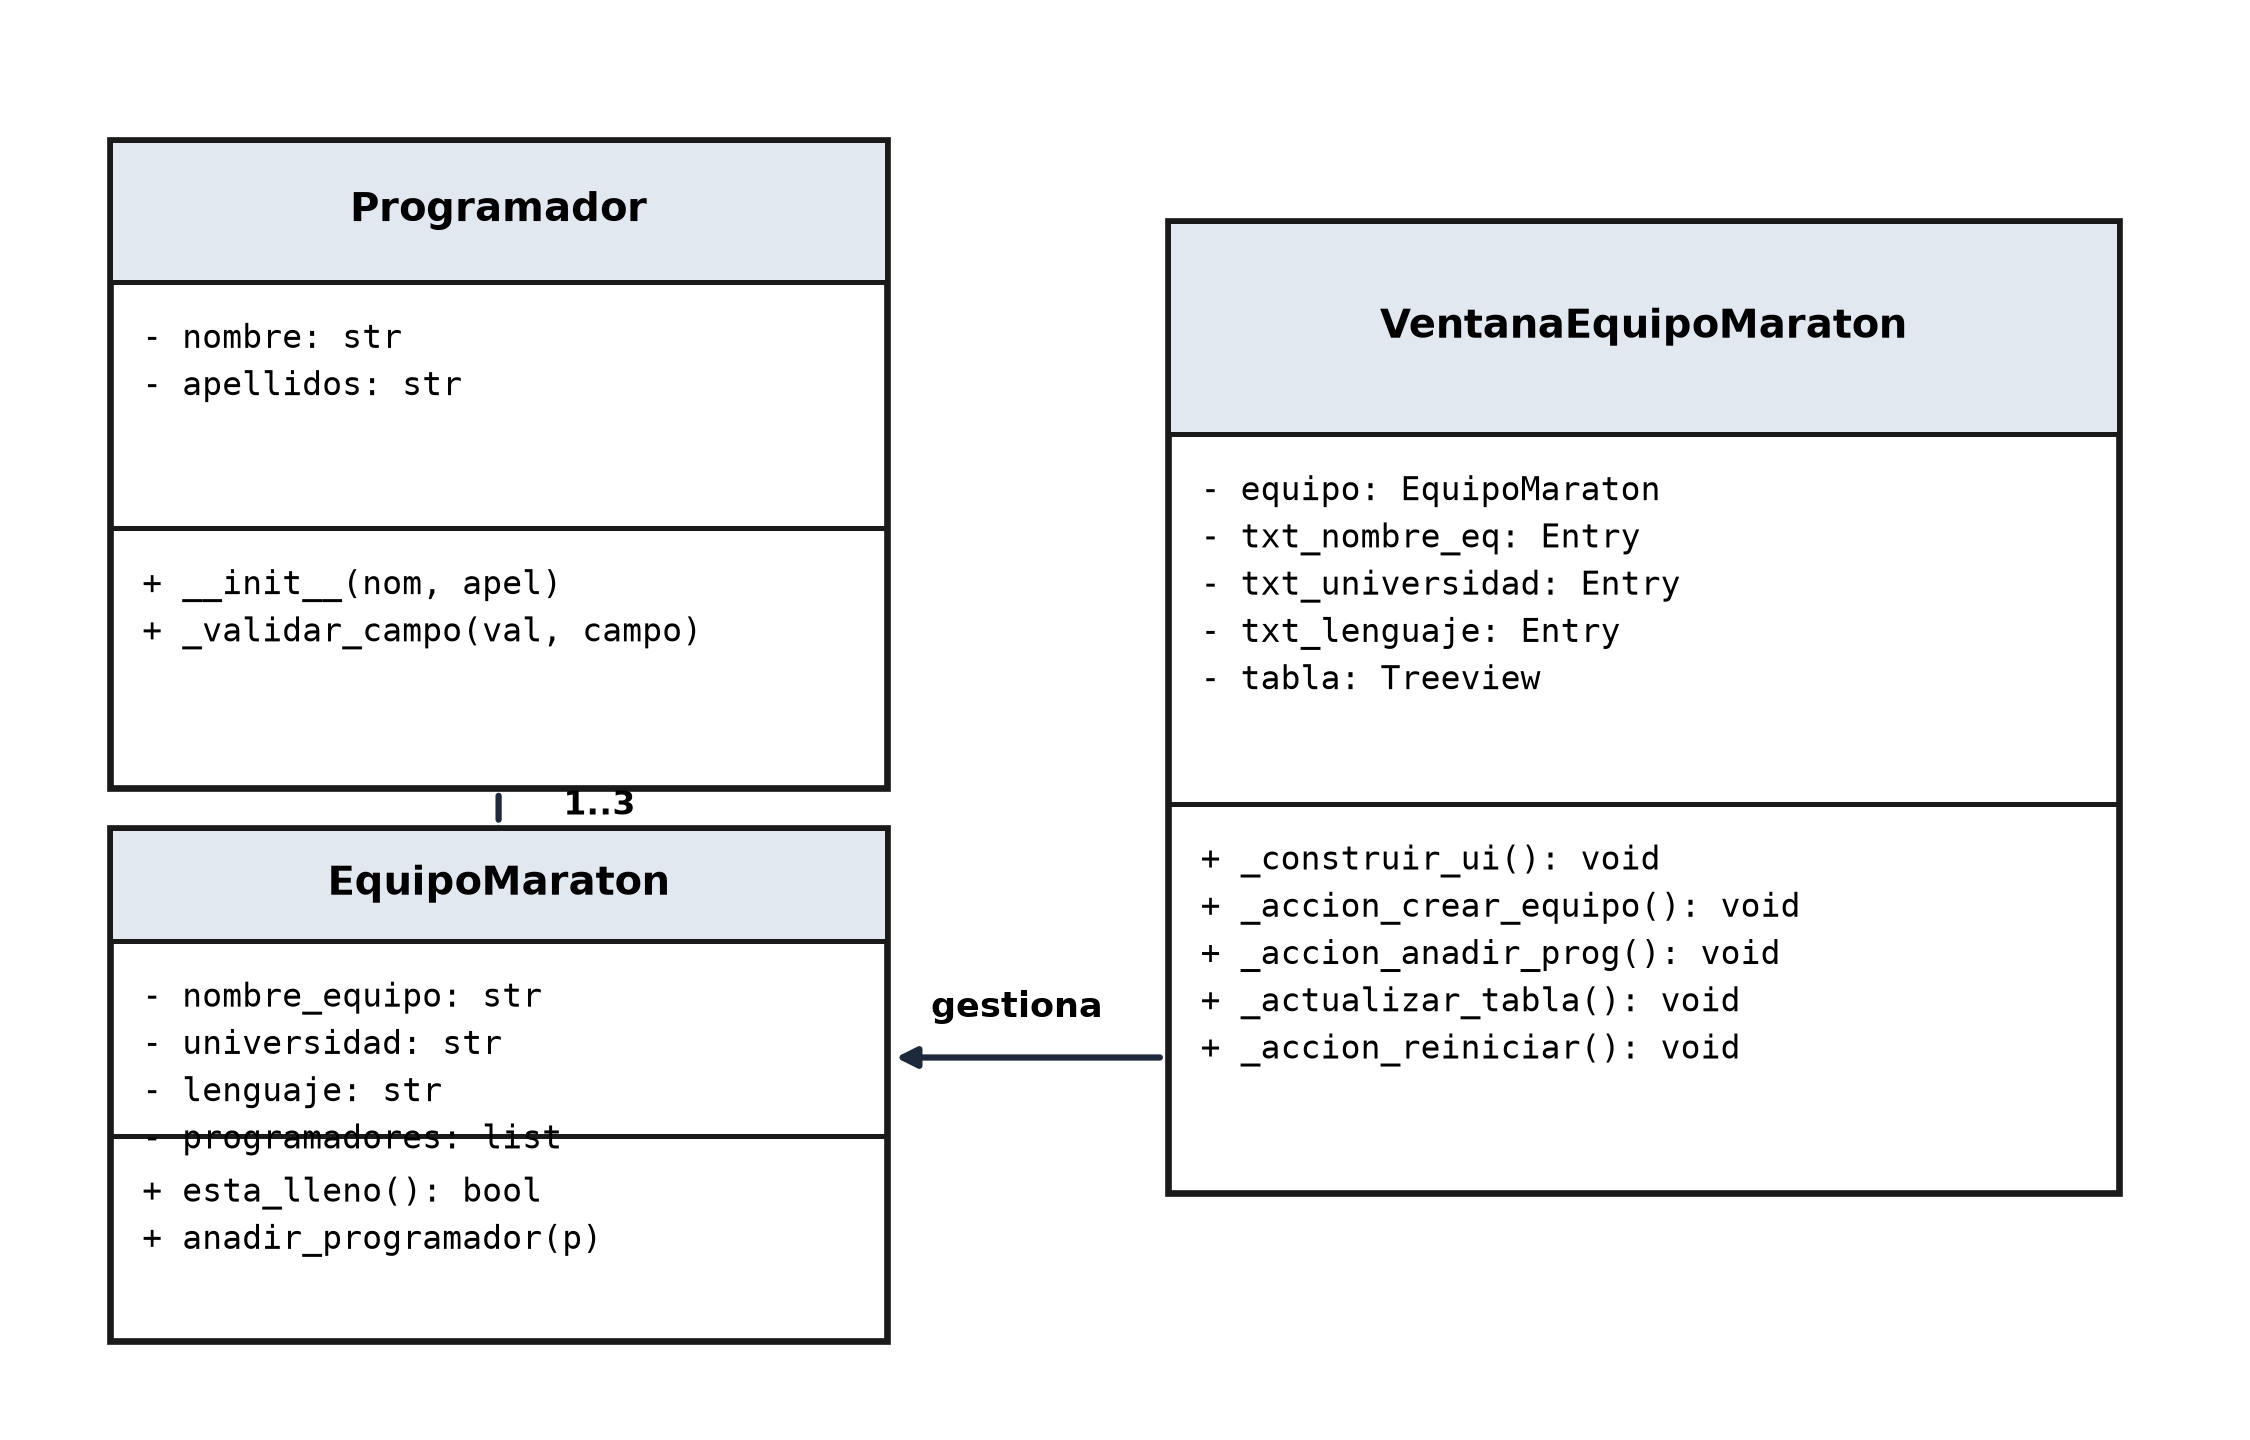
\includegraphics[width=0.82\textwidth]{figuras/clases_ejercicio6_7.png}
    \caption{Diagrama de clases para el ejercicio 6.7.}
    \label{fig:clases_67}
\end{figure}

\subsubsection{Casos de uso}
La figura \ref{fig:casos_67} recopila los casos de uso principales modelados para este módulo.

\begin{figure}[H]
    \centering
    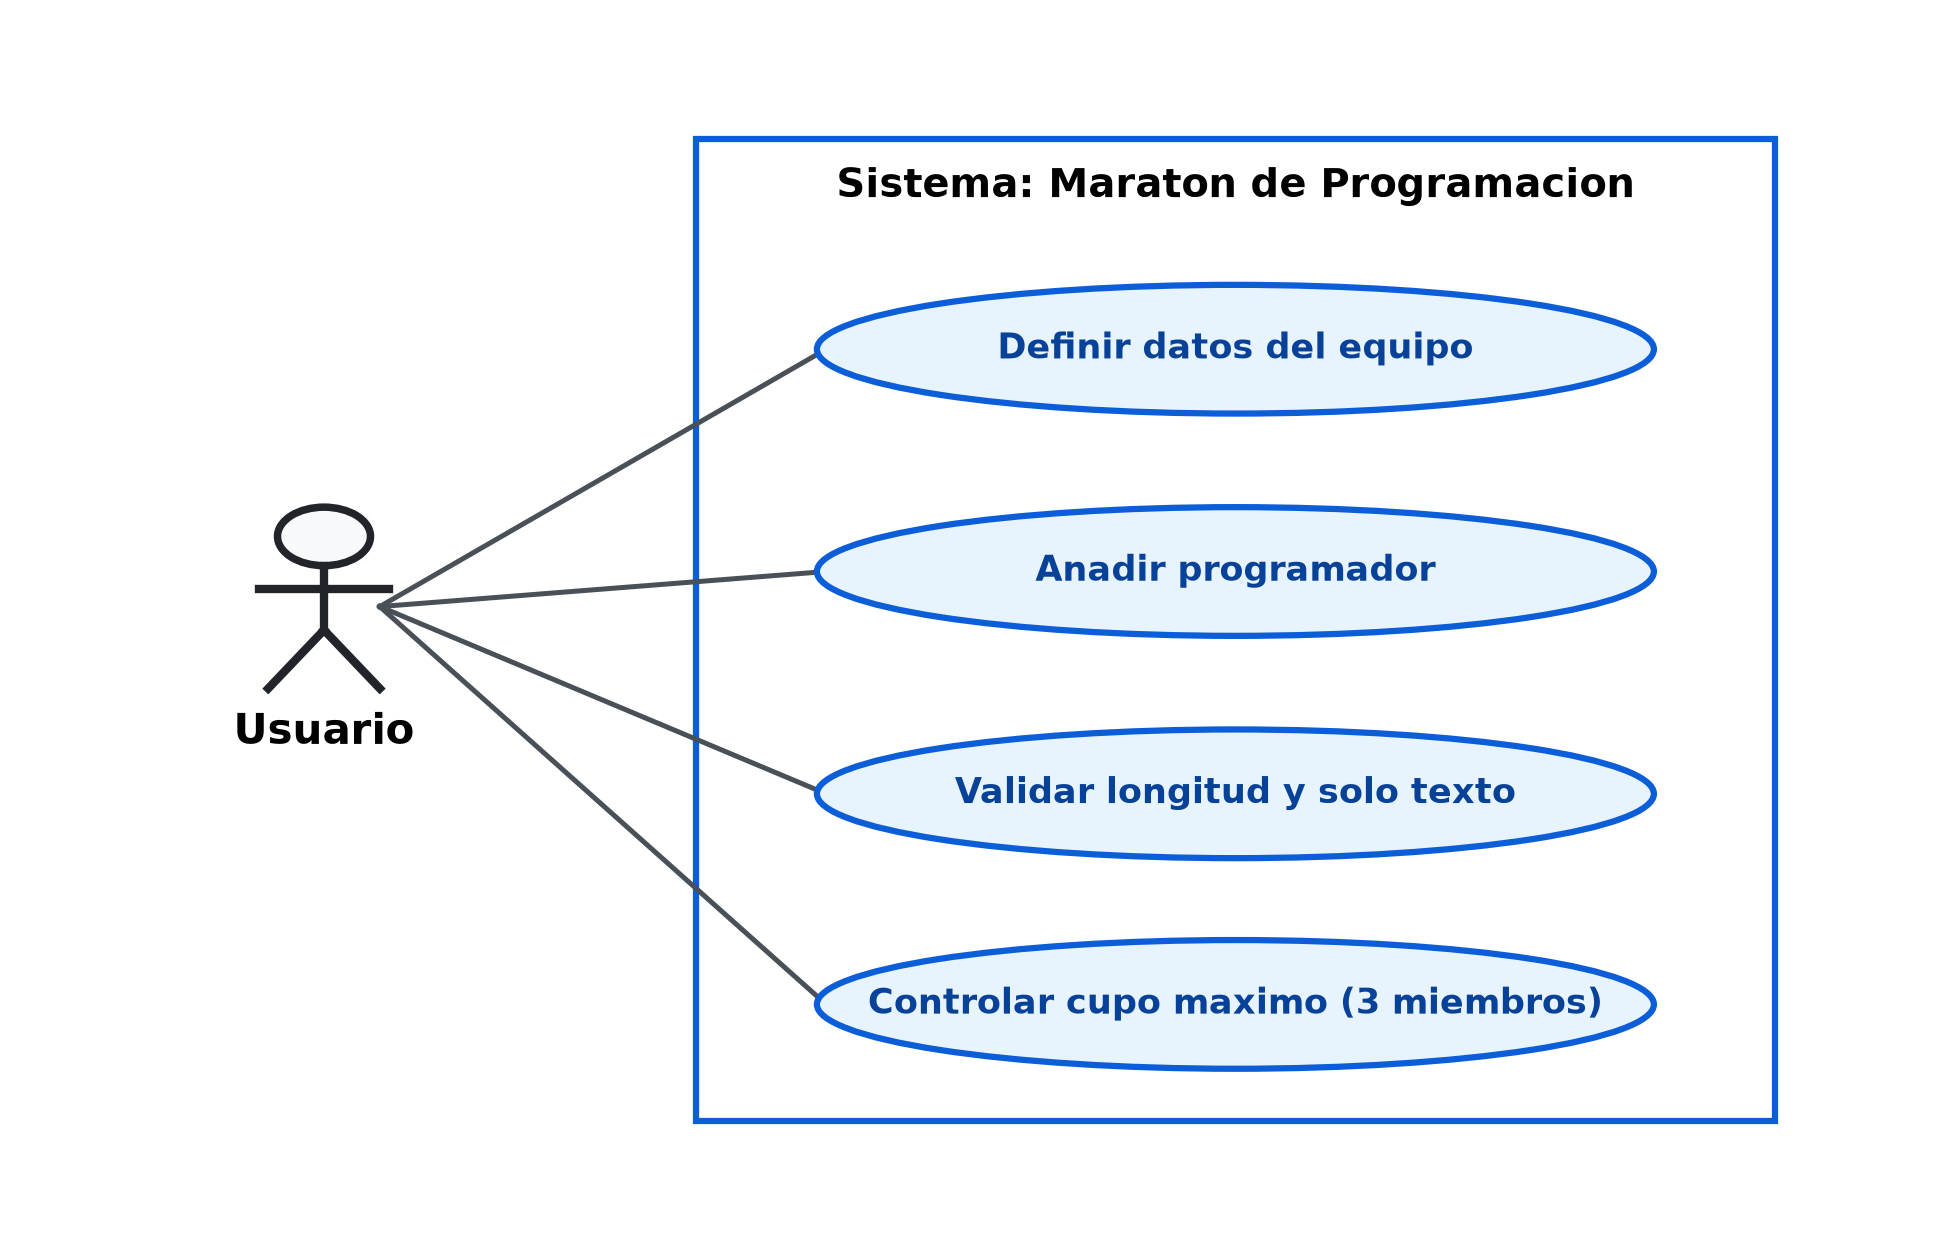
\includegraphics[width=0.75\textwidth]{figuras/casos_ejercicio6_7.png}
    \caption{Diagrama de casos de uso para el ejercicio 6.7.}
    \label{fig:casos_67}
\end{figure}

\begin{itemize}
    \item \textbf{Definir datos del equipo:} establece nombre, institución y lenguaje utilizado.
    \item \textbf{Añadir programador:} registra un miembro nuevo en la lista del equipo.
    \item \textbf{Validar longitud y solo texto:} comprueba que los nombres no contengan números y no excedan 20 caracteres.
    \item \textbf{Controlar cupo máximo (3 miembros):} genera una excepción controlada al superar la capacidad máxima admisible.
\end{itemize}

\clearpage

% ==============================================================================
% EJERCICIO 5
% ==============================================================================
\section{Ejercicio Página 427 (Ejercicio 6.8: Lectura de archivos)}

\noindent\textbf{Enlace a GitHub:} \\
\url{https://github.com/yguzmanm-sys/POO-2026-2S/blob/main/Actividad4/Ejercicio6_8.py}

\subsection{Descripción del Problema}
El ejercicio 6.8 del libro aborda la lectura secuencial de archivos de texto plano mediante flujos de bytes y caracteres (\texttt{FileInputStream}, \texttt{InputStreamReader} y \texttt{BufferedReader} en Java; context managers y flujos de lectura en Python) y el tratamiento de excepciones de entrada/salida (\texttt{FileNotFoundError}, \texttt{PermissionError} e \texttt{IOError}). Se implementó una solución visual que permite examinar archivos en el disco, cargar su contenido en un panel de texto con scroll, calcular estadísticas del archivo y convertir el texto a mayúsculas como propuesta de extensión del libro.

\subsection{Código Fuente}

\begin{lstlisting}[language=Python, caption=Lectura de archivos de texto con GUI en Python, label=lst:ej68]
import os
import tkinter as tk
from tkinter import ttk, filedialog, messagebox, scrolledtext

class LectorArchivo:
    @staticmethod
    def leer_archivo(ruta: str) -> tuple[str, int, int]:
        if not ruta.strip():
            raise ValueError("La ruta del archivo no puede estar vacia.")
        if not os.path.exists(ruta):
            raise FileNotFoundError(f"El archivo especificado no existe: {ruta}")
        if not os.path.isfile(ruta):
            raise IOError(f"La ruta indicada no corresponde a un archivo valido: {ruta}")

        try:
            with open(ruta, "r", encoding="utf-8") as archivo:
                lineas = archivo.readlines()
                contenido = "".join(lineas)
                total_lineas = len(lineas)
                total_caracteres = sum(len(linea) for linea in lineas)
                return contenido, total_lineas, total_caracteres
        except UnicodeDecodeError:
            with open(ruta, "r", encoding="latin-1") as archivo:
                lineas = archivo.readlines()
                contenido = "".join(lineas)
                return contenido, len(lineas), sum(len(linea) for linea in lineas)
        except PermissionError as e:
            raise PermissionError("Permiso denegado al intentar abrir el archivo.") from e
        except Exception as e:
            raise IOError(f"Ocurrio un error de entrada/salida al leer el archivo: {e}") from e

    @staticmethod
    def convertir_mayusculas(texto: str) -> str:
        return texto.upper()


class VentanaLeerArchivo(tk.Tk):
    def __init__(self):
        super().__init__()
        self.title("Ejercicio 6.8 - Lectura de Archivos")
        self.geometry("560x520")
        self.resizable(False, False)
        self.lector = LectorArchivo()
        self.contenido_cargado = ""
        self._construir_ui()

    def _construir_ui(self):
        marco = ttk.Frame(self, padding="15")
        marco.pack(fill=tk.BOTH, expand=True)

        lbl_titulo = ttk.Label(marco, text="Lectura y Visualizacion de Archivos de Texto", font=("Segoe UI", 12, "bold"))
        lbl_titulo.pack(pady=(0, 10))

        marco_ruta = ttk.LabelFrame(marco, text="Ubicacion del Archivo", padding="10")
        marco_ruta.pack(fill=tk.X, pady=5)

        self.txt_ruta = ttk.Entry(marco_ruta, width=42)
        self.txt_ruta.pack(side=tk.LEFT, padx=(0, 5), fill=tk.X, expand=True)

        btn_examinar = ttk.Button(marco_ruta, text="Examinar...", command=self._accion_examinar)
        btn_examinar.pack(side=tk.LEFT)

        marco_acciones = ttk.Frame(marco)
        marco_acciones.pack(fill=tk.X, pady=8)

        btn_leer = ttk.Button(marco_acciones, text="Leer Archivo", command=self._accion_leer)
        btn_leer.pack(side=tk.LEFT, padx=3)

        btn_mayus = ttk.Button(marco_acciones, text="A Mayusculas", command=self._accion_mayusculas)
        btn_mayus.pack(side=tk.LEFT, padx=3)

        btn_limpiar = ttk.Button(marco_acciones, text="Limpiar", command=self._accion_limpiar)
        btn_limpiar.pack(side=tk.LEFT, padx=3)

        ttk.Label(marco, text="Contenido del Archivo:", font=("Segoe UI", 10, "bold")).pack(anchor=tk.W, pady=(5, 2))
        self.txt_contenido = scrolledtext.ScrolledText(marco, width=64, height=14, font=("Consolas", 9))
        self.txt_contenido.pack(fill=tk.BOTH, expand=True)

        self.lbl_estado = ttk.Label(marco, text="Estado: Seleccione un archivo para comenzar.", font=("Segoe UI", 9))
        self.lbl_estado.pack(anchor=tk.W, pady=(6, 0))

    def _accion_examinar(self):
        ruta = filedialog.askopenfilename(
            title="Seleccionar archivo de texto",
            filetypes=[("Archivos de texto (*.txt)", "*.txt"), ("Todos los archivos", "*.*")]
        )
        if ruta:
            self.txt_ruta.delete(0, tk.END)
            self.txt_ruta.insert(0, ruta)

    def _accion_leer(self):
        ruta = self.txt_ruta.get().strip()
        try:
            contenido, lineas, caracteres = self.lector.leer_archivo(ruta)
            self.contenido_cargado = contenido
            self.txt_contenido.delete("1.0", tk.END)
            self.txt_contenido.insert(tk.END, contenido)
            self.lbl_estado.config(
                text=f"Lectura exitosa: {lineas} lineas, {caracteres} caracteres.",
                foreground="green"
            )
        except (ValueError, FileNotFoundError, PermissionError, IOError) as e:
            self.txt_contenido.delete("1.0", tk.END)
            self.lbl_estado.config(text=f"Error: {e}", foreground="red")
            messagebox.showerror("Error de Lectura", str(e))

    def _accion_mayusculas(self):
        if not self.contenido_cargado:
            messagebox.showwarning("Atencion", "No hay contenido cargado para transformar.")
            return
        texto_mayus = self.lector.convertir_mayusculas(self.contenido_cargado)
        self.txt_contenido.delete("1.0", tk.END)
        self.txt_contenido.insert(tk.END, texto_mayus)
        self.lbl_estado.config(text="Contenido transformado a mayusculas.", foreground="blue")

    def _accion_limpiar(self):
        self.txt_ruta.delete(0, tk.END)
        self.txt_contenido.delete("1.0", tk.END)
        self.contenido_cargado = ""
        self.lbl_estado.config(text="Estado: Formulario reiniciado.", foreground="black")


if __name__ == "__main__":
    app = VentanaLeerArchivo()
    app.mainloop()
\end{lstlisting}

\subsection{Interfaz de usuario}
La figura \ref{fig:ui_68} muestra la ventana desarrollada para la lectura de archivos. Incorpora un selector con diálogo de navegación en el sistema de ficheros, botones de lectura, conversión a mayúsculas y limpieza, un visor con barra de desplazamiento para visualizar el contenido y una barra de estado informativa.

\begin{figure}[H]
    \centering
    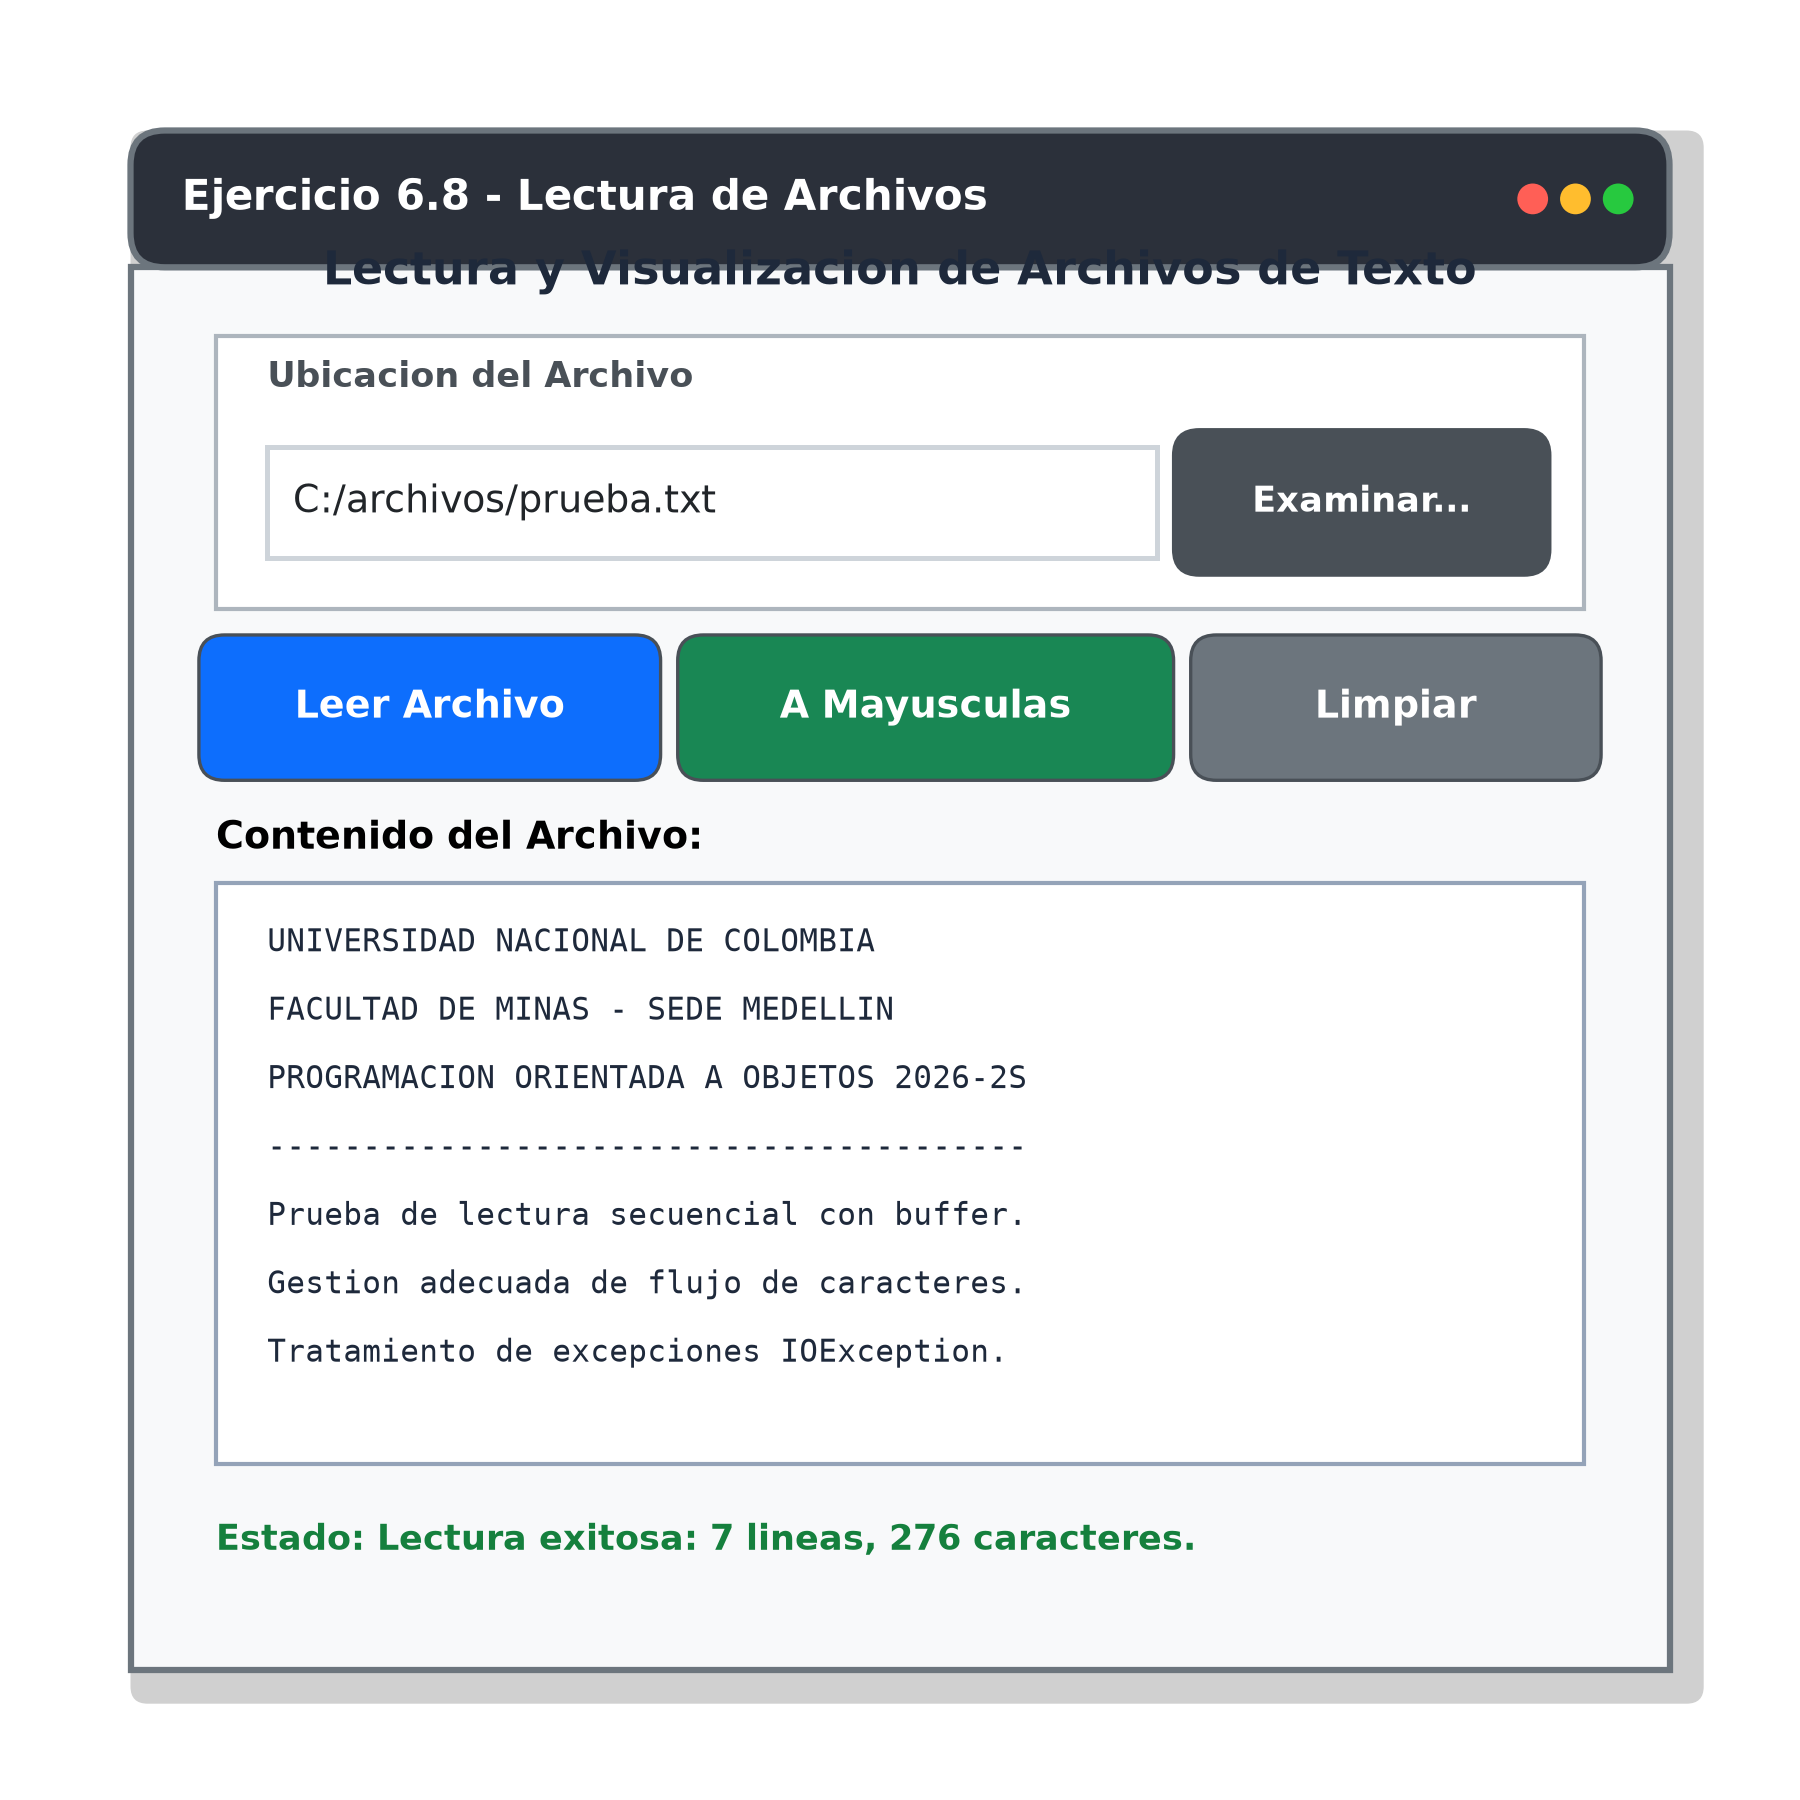
\includegraphics[width=0.55\textwidth]{figuras/ui_ejercicio6_8.png}
    \caption{Interfaz de usuario para el ejercicio 6.8 (Página 427).}
    \label{fig:ui_68}
\end{figure}

\subsection{Diagramas UML}

\subsubsection{Diagrama de clases}
El diagrama de clases de la figura \ref{fig:clases_68} describe la clase \texttt{LectorArchivo}, encargada de gestionar los flujos de lectura en disco y tratamiento de excepciones de E/S, y la clase \texttt{VentanaLeerArchivo}, responsable de la interacción visual con el usuario.

\begin{figure}[H]
    \centering
    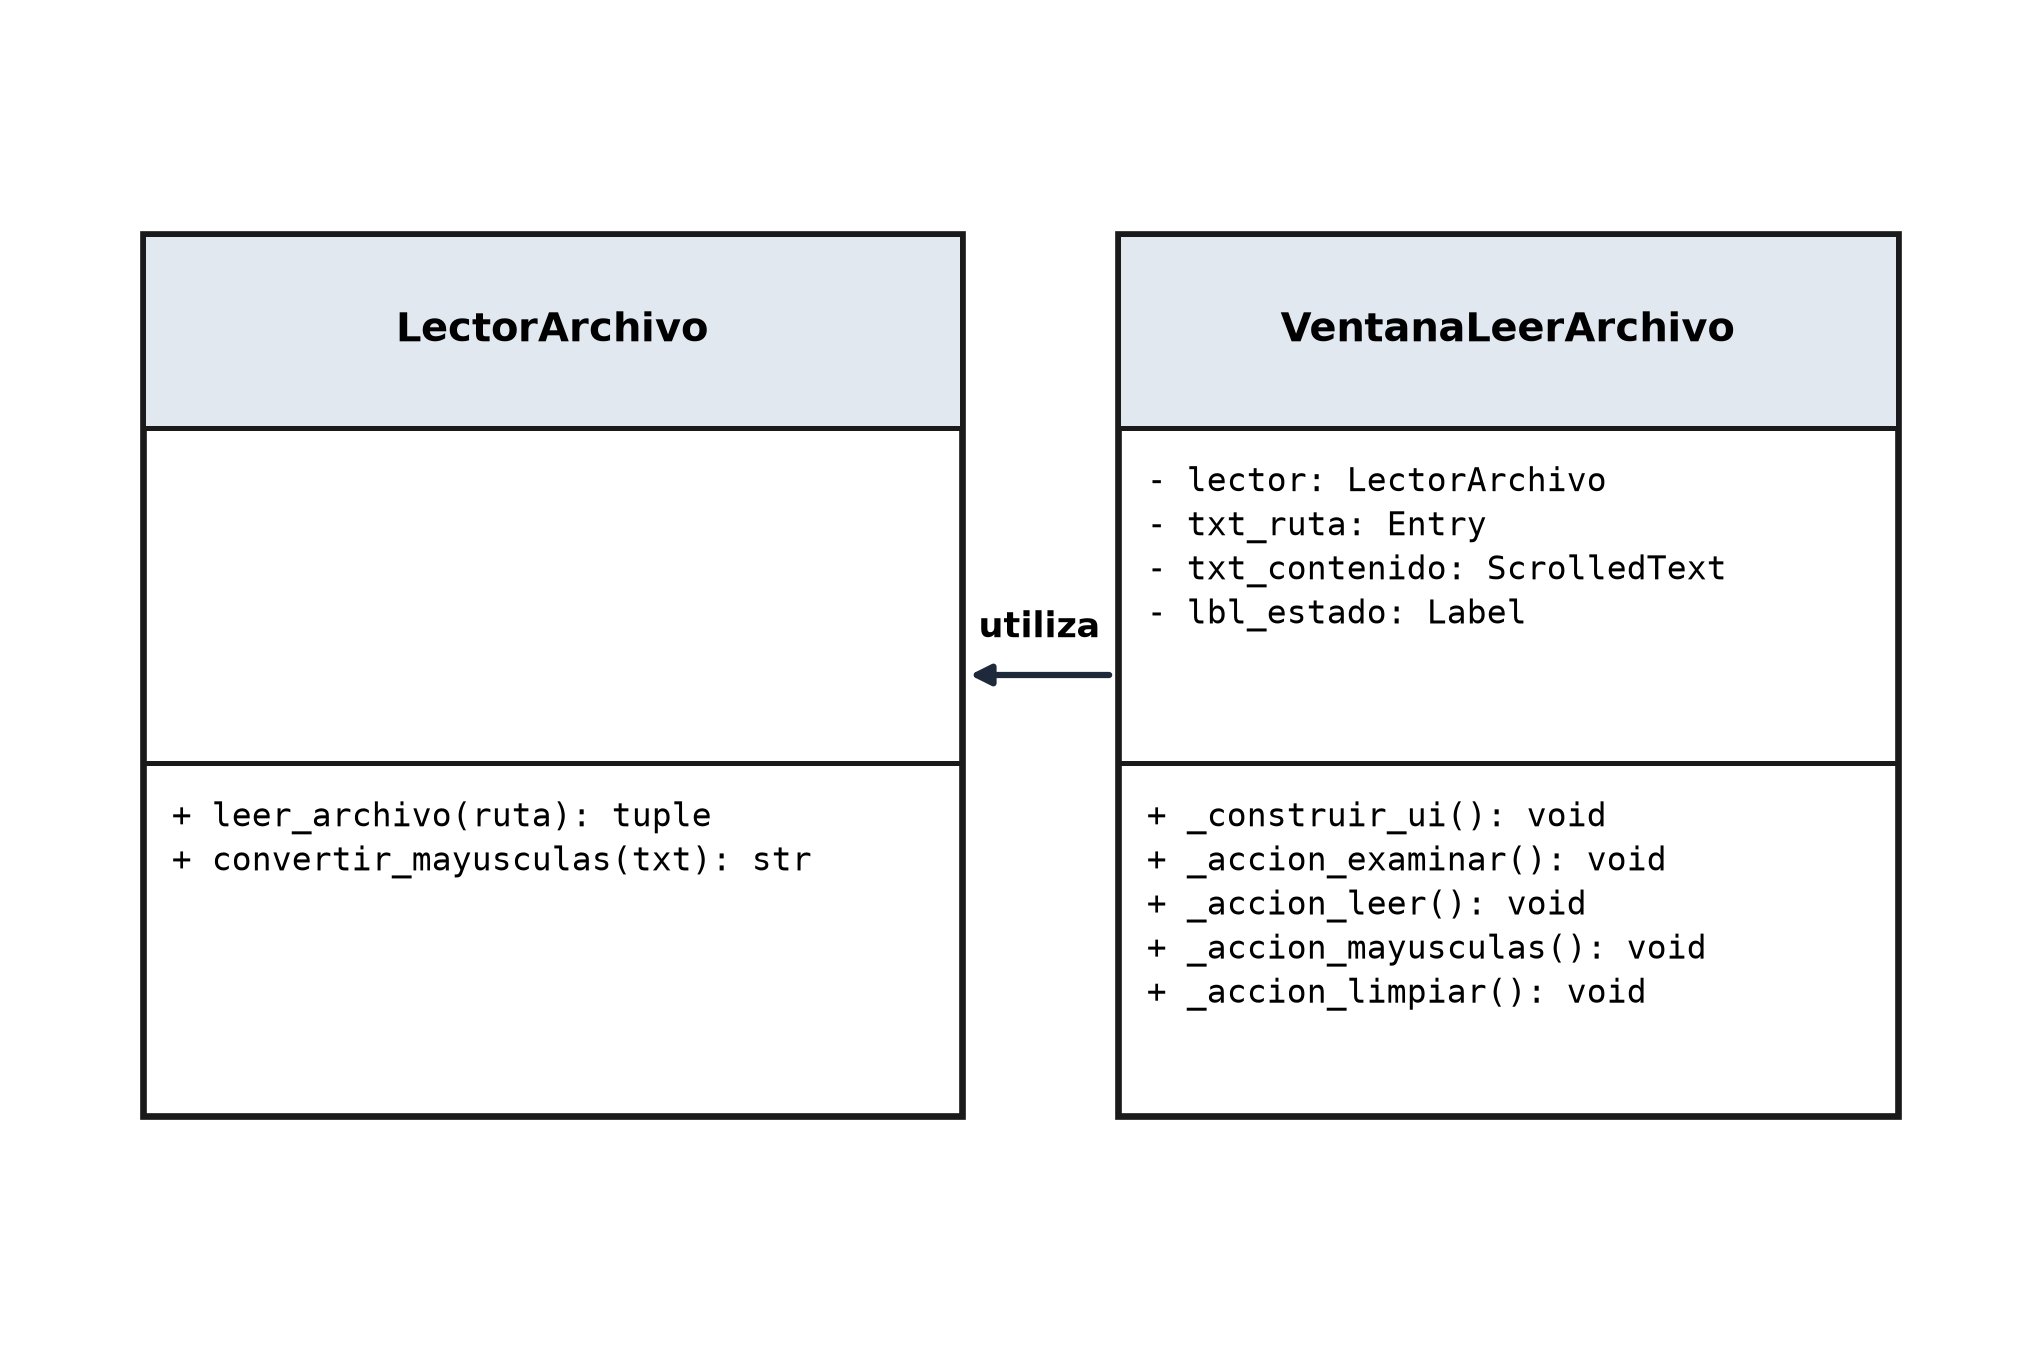
\includegraphics[width=0.78\textwidth]{figuras/clases_ejercicio6_8.png}
    \caption{Diagrama de clases para el ejercicio 6.8.}
    \label{fig:clases_68}
\end{figure}

\subsubsection{Casos de uso}
La figura \ref{fig:casos_68} resume los casos de uso modelados para la gestión y lectura de archivos.

\begin{figure}[H]
    \centering
    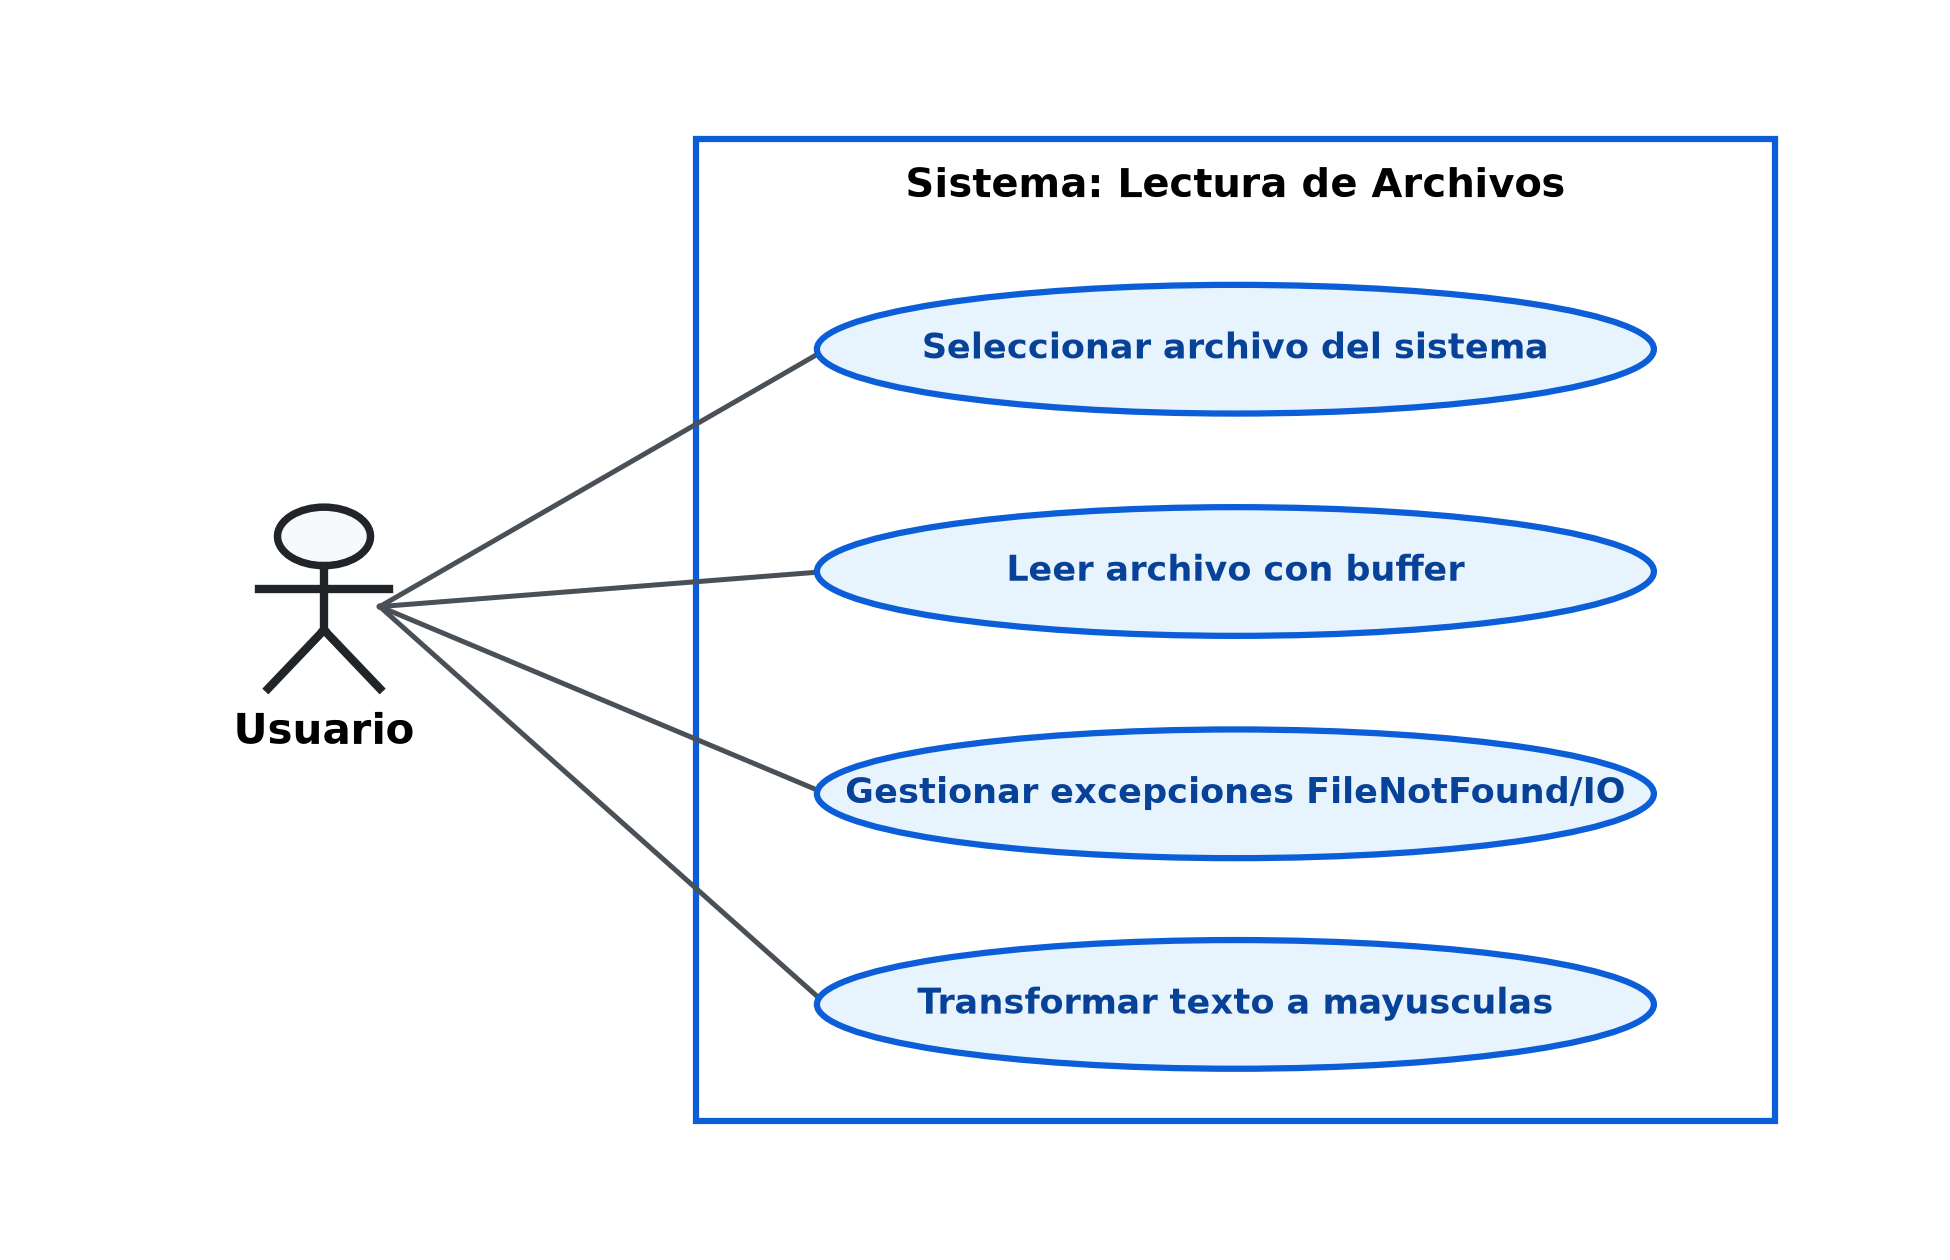
\includegraphics[width=0.75\textwidth]{figuras/casos_ejercicio6_8.png}
    \caption{Diagrama de casos de uso para el ejercicio 6.8.}
    \label{fig:casos_68}
\end{figure}

\begin{itemize}
    \item \textbf{Seleccionar archivo del sistema:} navegación mediante el explorador para elegir el archivo \texttt{.txt}.
    \item \textbf{Leer archivo con buffer:} carga secuencial del contenido con cierre seguro del flujo de datos.
    \item \textbf{Gestionar excepciones FileNotFound/IO:} captura de condiciones donde el archivo no existe o se carece de permisos de lectura.
    \item \textbf{Transformar texto a mayúsculas:} manipulación del flujo de texto cargado en pantalla.
\end{itemize}

\end{document}
